\documentclass[10pt,final,hidelinks]{article}
\usepackage{lmodern}
\usepackage[T1]{fontenc}
\usepackage[english]{babel}
\usepackage[utf8]{inputenc}
\usepackage[activate={true,nocompatibility},final,tracking=true,kerning=true,
    spacing=true,factor=1100,stretch=10,shrink=10]{microtype}
\microtypecontext{spacing=nonfrench}
\usepackage[margin=.5in]{geometry}
\usepackage{graphicx}
\graphicspath{{img/}} 
\usepackage[noend]{algorithm2e}
\usepackage{caption}
\usepackage{subcaption}
\usepackage{booktabs}
\usepackage{array}
\usepackage{mathtools}
\usepackage{subfiles}
\usepackage{enumitem}
\usepackage{commath}
\usepackage{appendix}
\renewcommand\appendixtocname{Appendices}
\usepackage{amsmath}
\usepackage{amsthm}
\usepackage{amssymb}
%\usepackage[intoc,english]{nomencl}
%\makenomenclature
\usepackage{pgfplots}
\usepackage{tabu} 
\usepackage{tikz}
\usepackage{tikzscale}
\usepackage[square,numbers]{natbib}
\bibliographystyle{plain}
\usepackage{siunitx}
\numberwithin{equation}{section}
\usepackage{hyperref}
\usepackage{cleveref}

\pgfplotsset{compat=newest}

\newcommand{\COMMENT}[1]{}

\usepackage{custom}
\usepackage{algorithmnotation}
\usepackage{matrixnotation}
\usepackage[fancy]{setnotation}
\usepackage[fancy]{relationnotation}
\usepackage{approxsetnotation}
\usepackage{approxrelationnotation}
\usepackage[section]{envnotation}

\hypersetup{
    pdftitle={First-order random approximate set model
    and corresponding binary classification measures modeled as random variables.},
    pdfauthor={Alexander Towell},               % author
    pdfsubject={computer science},              % subject of the %document
    pdfkeywords={
        probabilistic data structure,
        abstract data type,
        approximate set,
        bloom filter,
        perfect hash function,
        perfect hash filter},                   % keywords
    colorlinks=true,                            % false: boxed links;
    linkcolor=magenta,
    citecolor=green,                            % color of links to 
    filecolor=blue,                             % color of file links
    urlcolor=green                              % color of external
}

\title
{
    First-order random approximate set model\\
    \large and corresponding random binary classification measures.
}
\author
{
    Alexander Towell\\
    \texttt{atowell@siue.edu}
}
\date{}

\begin{document}
\maketitle
\begin{abstract}
We define a \emph{random approximate set} model and the probability space that 
follows.
A random approximate set is a \emph{probabilistic} set generated to \emph{approximate} another set of objective interest.
We derive several properties that follow from this definition, such as the expected \emph{precision} in information retrieval.
Finally, we demonstrate an application of approximate sets, approximate Encrypted Search with queries as a Boolean algebra, which generates random approximate result sets.
\end{abstract}

%\microtypesetup{protrusion=false}
\tableofcontents
%\microtypesetup{protrusion=true}
%\listoftables
%\listoffigures

%\nomenclature{$\vec{x}$}{Vectors are denoted in boldface font. The \jth component of $\vec{x}$ is denoted by $x_j$.}

\nomenclature[S]{$\Set{S}$}{Sets are normally notated like this.}
\nomenclature[S]{$\RealSet$}{The set of reals $(-\infty,\infty)$.}
\nomenclature[S]{$\NatSet$}{The set of natural numbers $\{0,1\}$.}
\nomenclature[S]{$\BitSet$}{The binary set $\{0,1\}$.}
\nomenclature[S]{$\Set{A}_{p}$}{The set $\SetBuilder{a \in \Set{A}}{\operatorname{p}(a)}$ where $\operatorname{p} \colon \Set{U} \mapsto \{0,1}$ is a predicate function over some universal set.}

\nomenclature[R]{$\ASet{A}$}{A \emph{random approximate set} of $\Set{A}$ where the false positive and negative rates are unspecified.}
%\nomenclature[R]{$\ASet{A}[\tprate][\fprate]$}{A \emph{random approximate set} of $\Set{A}$ where the parameterizations are $\tprate$ and $\fprate$.}
\nomenclature[R]{$\ASet{A}[\fnrate][\fprate]$}{A \emph{random approximate set} of $\Set{A}$ where the parameterizations are $\fnrate$ and $\fprate$.}
%\nomenclature[R]{$\ASet{A}[\tprate][+]$}{A \emph{random approximate set} of $\Set{A}$ where the false positive rate is unspecified or implicit.}
\nomenclature[R]{$\ASet{A}[\fnrate][+]$}{A \emph{random approximate set} of $\Set{A}$ where the false positive rate is unspecified.}
\nomenclature[R]{$\ASet{A}[-][\fprate]$}{A \emph{random approximate set} of $\Set{A}$ where the true positive rate is unspecified.}
\nomenclature[R]{$\ASet{A}[-][\tnrate]$}{A \emph{random approximate set} of $\Set{A}$ where the false negative rate is unspecified.}
\nomenclature[R]{$\PASet{A}$}{A \emph{positive} random approximate set of $\Set{A}$ where the false positive rate is unspecified.}
\nomenclature[R]{$\PASet{A}[\fprate]$}{A \emph{positive} random approximate set of $\Set{A}$ where the false positive rate is $\fprate$.}
\nomenclature[R]{$\NASet{A}$}{A \emph{negative} random approximate set of $\Set{A}$ where the true positive rate is unspecified.}
%\nomenclature[R]{$\NASet{A}[\tprate]$}{A \emph{negative} random approximate set of $\Set{A}$ where the true positive rate is $\tprate$.}
\nomenclature[R]{$\NASet{A}[\fnrate]$}{A \emph{negative} random approximate set of $\Set{A}$ where the false negative rate is $\fnrate$.}

\nomenclature[R]{$\fprate$}{By convention, an \emph{expected} false positive rate if nothing about it is known.}
\nomenclature[R]{$\tprate$}{By convention, an \emph{expected} true positive rate if nothing about it is known.}
\nomenclature[R]{$\tnrate$}{By convention, an \emph{expected} true negative rate if nothing about it is known.}
\nomenclature[R]{$\fnrate$}{By convention, an \emph{expected} false negative rate if nothing about it is known.}

\nomenclature[R]{$\fprateob$}{By convention, an \emph{observed} false positive rate if nothing about it is known.}
\nomenclature[R]{$\tprateob$}{By convention, an \emph{observed} true positive rate if nothing about it is known.}
\nomenclature[R]{$\tnrateob$}{By convention, an \emph{observed} true negative rate if nothing about it is known.}
\nomenclature[R]{$\fnrateob$}{By convention, an \emph{observed} false negative rate if nothing about it is known.}

\nomenclature[T]{$\Card{\Set{A}}$}{The cardinality of a set $\Set{A}$.}
\nomenclature[T]{$\Set{A} \times \Set{B}$}{The Cartesian product of $\Set{A}$ and $\Set{B}$ defined as $\SetBuilder{\Pair{a}{b}}{a \in \Set{A} \land b \in \Set{B}}$.}
\nomenclature[T]{$\Set{B}^n$}{The Cartesian product $\Set{B} \times \cdots \times \Set{B}$, $n$ times.}
\nomenclature[T]{$\SetIndicator{}$}{The indicator function, $\SetIndicator{\Set{A}} \colon \Set{X} \mapsto \{0,1\}$ is defined by $\SetIndicator{\Set{A}}(x) = 1$ if $x \in \Set{A}$ and otherwise equals $0$.}
\nomenclature[T]{$\PowerSet(A)$}{The power set of $\Set{A}$.}
\nomenclature[T]{$\PS{A}$}{The power set of $\Set{A}$.}
\nomenclature[T]{$\SetUnion[\Set{A}][\Set{B}]$}{The union of $\Set{A}$ and $\Set{B}$.}
\nomenclature[T]{$\SetUnion[\ASet{A}][\ASet{B}]$}{The union of random approximate sets $\ASet{A}$ and $\ASet{B}$.}

\nomenclature[P]{$\PDF[\RV{X}]$}{The probability mass or density function of random variable $\RV{X}$.}
\nomenclature[P]{$\CDF[\RV{X}]$}{The cumulative distribution function of random variable $\RV{X}$.}

\nomenclature{$\BL$}{The bit length function.}
\nomenclature{$\RE$}{The relative efficiency function.}
\nomenclature{$\AbsoluteEfficiency$}{The absolute efficiency function.}


%\printnomenclature

\subfile{sections/intro}
\subfile{sections/algebra_of_sets}
\subfile{sections/aset_model}
\subfile{sections/first_order_model}
\subfile{sections/derived_distributions}
\subfile{sections/relational}
\subfile{sections/aset_theory}
\subfile{sections/interval}
\subfile{sections/aset_adt}
\subfile{sections/appendix}

\bibliography{references}

\end{document}
\documentclass[ ../main.tex]{subfiles}
\providecommand{\mainx}{..}
\begin{document}
\section{Introduction}
% the queries may also be rate distorted. or approximate.

%The (approximate) logical functions $\land \colon \Bool^{\fnrate}_{\fprate} \times \Bool^{\fnrate}_{\fprate} \mapsto \Bool^{\fnrate}_{\fprate}$ and $\neg \colon \Bool^{\fnrate}_{\fprate} \mapsto \Bool^{\fnrate}_{\fprate}$ are also random, e.g., assuming $\neg$ does not introduce an \emph{independent} source of error, $\neg \True^{\fnrate}$ and $\neg \False^{\fprate}$ are respectively distributed as $\False^{\fnrate}$ and $\True^{\tprate}$.

An \emph{approximate set} is a set that approximates another set of objective interest.
It is \emph{approximate} because with respect to the objective set, there are two types of errors, \emph{false positives} and \emph{false negatives}.
The \emph{Bloom filter} is a popular example of a data structure that models \emph{positive random approximate sets} with \emph{false positives} due to \emph{rate distortion}.

In \cref{sec:setalgebra}, we define the algebra of sets.

In \cref{sec:asets}, we provide a formal definition of the \emph{random approximate set} model, in which the false positive and false negative rates are \emph{expectations}.
We describe the axioms of the random approximate set model such that, if satisfied, also satisfy the axioms of the approximate algebra of sets.
We further derive the probability distribution of random approximate sets entailed by the axioms.

In \cref{sec:characteristics}, we derive the rate-distortion random variables that are fundamental to the approximate set model, such as the false positive rate.

In \cref{sec:func_rand_asets}, we provide a detailed treatment on distributions that are induced by functions that depend on random approximate sets, e.g., in \cref{sec:set_theory} we derive the probability distribution of random approximate sets that are generated from arbitrary set-theoretic operations on random approximate sets and in \cref{sec:perf} we derive several well-known binary classification performance measures of random approximate sets as a function of their error rates, such as \emph{positive predictive value}.

In \cref{sec:intervals}, we provide the probabilistic model for random approximate sets with \emph{uncertain} rate distortions, such as an uncertain false positive rate.

In \cref{sec:adt}, we provide a treatment on the random approximate set model as an abstract data type and show how that, if the generative algorithm of an approximate set model is deterministic, the random approximate set model quantifies our ignorance or uncertainty.

Finally, in \cref{sec:bool_search}, we consider Encrypted Search with secure indexes based on random approximate sets.
To prove various properties of this model, such as expected precision, we only need to show that the \emph{result sets} are approximate sets of the \emph{objective} results and all the results immediately follow.
\end{document}\documentclass[../main.tex]{subfiles}
\providecommand{\mainx}{..}
\begin{document}
\section{Algebra of sets} 
\label{sec:setalgebra}
A \emph{set}\index{set} is an unordered collection of distinct elements.
If we know the elements in a set, we may denote the set by these elements, e.g., $\{a,c,b\}$ denotes a set whose members are exactly $a$, $b$, and $c$.

Two sets of particular importance are the empty set, denoted by $\EmptySet$, which has no members, and the \emph{universal set}, in which every element of interest is a member.

A \emph{finite set} has a finite number of elements.
For example, $\{ 1, 3, 5 \}$ is a finite set with three elements.
When sets $\Set{A}$ and $\Set{B}$ are \emph{isomorphic}, denoted by $\Set{A} 
\cong \Set{B}$, they can be put into a one-to-one correspondence (bijection), e.g., $\{b,a,c\} \cong \{1,2,3\}$.

The cardinality of a finite set $\Set{A}$ is the number of elements in the set, denoted by $\Card{\Set{A}}$, e.g., $\Card{\left\{ 1, 3, 5\right\}} = 3$.
A \emph{countably infinite set} is isomorphic to the set of \emph{natural numbers} $\NatSet \coloneqq \{1,2,3,4,5,\ldots\}$.


Given two elements $a$ and $b$, an ordered pair of $a$ then $b$ is denoted by $\Pair{a}{b}$, where $\Pair{a}{b} = \Pair{c}{d}$ \emph{if and only if} $a = c$ and $b = d$.
Ordered pairs are non-commutative and non-associative, i.e., $\Pair{a}{b} \neq \Pair{b}{a}$ if $a \neq b$ and $\Pair{a}{\Pair{b}{c}} \neq \Pair{\Pair{b}{a}}{c}$.

Related to the ordered pair is the Cartesian product.
\begin{definition}
	The set $\Set{X} \times \Set{Y} \coloneqq \left\{\Pair{x}{y} \colon x \in 
	\Set{X} \land y \in \Set{Y}\right\}$ is the Cartesian product of sets $\Set{X}$ 
	and $\Set{Y}$.
\end{definition}
By the non-commutative and non-associative property of ordered pairs, the Cartesian product is non-commutative and non-associative.
However, they are isomorphic, i.e., $\Set{X} \times \Set{Y} \cong \Set{Y} \times \Set{X}$.

A \emph{tuple} is a generalization of order pairs which can consist of an arbitrary number of elements, e.g., $\Tuple{x_1,x_2,\ldots,x_n}$.
\begin{definition}[$n$-fold Cartesian product]
	The $n$-ary Cartesian product of sets $\Set{X}[1],\ldots,\Set{X}[n]$, is given by $\Set{X}[1] \times \cdots \times \Set{X}[n] = \left\{\Tuple{x_1,\ldots,x_n} \colon x_1 \in \Set{X}[1] \land \cdots \land x_n \in \Set{X}[n]\right\}$.
\end{definition}
Note that
	$\Set{X}[1] \times \Set{X}[2] \times \Set{X}[3] \cong \Set{X}[1] \times \left(\Set{X}[2] \times \Set{X}[3]\right) \cong \left(\Set{X}[1] \times \Set{X}[2]\right) \times \Set{X}[3]$,
thus we may implicitly convert between them without ambiguity.

If each set in the $n$-ary Cartesian product is the same, the power notation may be used, e.g., $\Set{X}^3 \coloneqq \Set{X} \times \Set{X} \times \Set{X}$.
As special cases, $\Set{X}^0 \coloneqq \{ \EmptySet \}$ and $\Set{X}^1 \coloneqq \Set{X}$.

A \emph{binary relation} over sets $\Set{A}$ and $\Set{B}$ is any subset of $\Set{A} \times \Set{B}$.
A fundamental relation is the member-of relation, where $\SetContains[x][\Set{A}]$ denotes that an object $x$ is a member of a set $\Set{A}$.
A set $\Set{A}$ is a \emph{subset} of a set $\Set{B}$ if every member of $\Set{A}$ is a member $\Set{B}$, denoted by $\Set{A} \subseteq \Set{B}$.
The subset relation forms a \emph{partial order}, i.e., if $\Set{A} \subseteq \Set{B}$ and $\Set{B} \subseteq \Set{C}$ then $\Set{A} \subseteq \Set{C}$ and 
if $\Set{A} \subseteq \Set{B}$ and $\Set{B} \subseteq \Set{A}$ then $\Set{A}$ and $\Set{B}$ are \emph{equal}, denoted by $\Set{A} = \Set{B}$.


\begin{definition}
	Set builder notation
\end{definition}


\begin{definition}
	A \emph{function} of type $\Set{X} \mapsto \Set{Y}$ is a binary relation on $\Set{X} \times \Set{Y}$ with the constraint that each $x \in \Set{X}$ is paired with exactly one $y \in \Set{Y}$.
\end{definition}
A function of type $\Set{X} \mapsto \Set{Y}$ has a domain $\Set{X}$ and a codomain $\Set{Y}$.
Since every $x \in \Set{X}$, given a pair $\Pair{x}{y} \in \Fun{f}$, $y$ may also be denoted by $\Fun{f}(x)$.

The \emph{power set} of a set $\Set{A}$, denoted by $\PS{\Set{A}}$, is the set of sets that contains all of the possible subsets of $\Set{A}$, e.g., $\PS{\{a, b\}}= \left\{ \EmptySet, \{a\}, \{b\}, \{a, b\} \right\}$.

A predicate is a function that maps elements in its domain to true (denoted by $1$) or false (denoted by $0$).
A predicate function of particular importance is the indicator function
\begin{equation}
	\SetIndicator{\Set{A}} \colon \Set{X} \mapsto \{0,1\}
\end{equation}
defined as
\begin{equation}
	\SetIndicator{\Set{A}}(x) \coloneqq
	\begin{cases}
		0 & \text{if $x \notin \Set{A}$}\,,\\
		1 & \text{if $x \in \Set{A}$}\,.
	\end{cases}
\end{equation}

The indicator function admits the construction of predicates for any relation, e.g., a binary predicate $\operatorname{P}$ for a binary relation $\Set{R} \subseteq \Set{A} \times \Set{B}$ is defined as $\operatorname{P}(x_1,x_2) \coloneqq \SetIndicator{\Set{R}}(\Pair{x_1}{x_2})$.
Denoting the \emph{universal set} by $\Set{X}$, all the relations mentioned previously are \emph{binary predicates}, such as $\SetContains \colon \Set{X} \times \PS{\Set{X}} \mapsto \{0,1\}$ and $\subseteq \colon \PS{\Set{X}} \times \PS{\Set{X}} \mapsto \{0,1\}$.

A few important operations on sets are \emph{set-union} $\SetUnion \colon \PS{\Set{X}} \times \PS{\Set{X}} \mapsto \PS{\Set{X}}$, \emph{set-intersection}, $\SetIntersection \colon \PS{\Set{X}} \times \PS{\Set{X}} \mapsto \PS{\Set{X}}$, and \emph{set-complement} $\SetComplement \colon \PS{\Set{X}} \mapsto \PS{\Set{X}}$, respectively defined as
\begin{align}
	\SetUnion[\Set{A}][\Set{B}]			&\coloneqq \SetBuilder{ x \in \Set{X}}{x \in \Set{A} \lor x \in \Set{B}}\,,\\
	\SetIntersection[\Set{A}][\Set{B}]	&\coloneqq \SetBuilder{ x \in \Set{X}}{x \in \Set{A} \land x \in \Set{B}}\,,\,\text{and}\\
	\SetComplement[\Set{A}]				&\coloneqq \SetBuilder{ x \in \Set{X}}{x \notin \Set{A}}\,.
\end{align}
where $\lor$ and $\land$ are respectively the logical-connectives \emph{or} and \emph{and}.
If $\SetIntersection[\Set{A}][\Set{B}] = \EmptySet$, then we say $\Set{A}$ and $\Set{B}$ are \emph{disjoint} sets.
\end{document}\documentclass[ ../main.tex]{subfiles}
\providecommand{\mainx}{..}
\begin{document}
\section{Approximate sets}
\label{sec:asets}
Given an objective set $\Set{A}$, any element that is a member of $\Set{A}$ is denoted a \emph{positive} (of $\Set{A})$ and otherwise the element is denoted a \emph{negative}.
Suppose $\hat{\Set{A}}$ is used as an \emph{approximation} of $\Set{A}$.
If the \emph{only} information we have about $\Set{A}$ is given by $\hat{\Set{A}}$, then we may perform membership tests on $\hat{\Set{A}}$ to make \emph{predictions} or \emph{estimations} about $\Set{A}$.

There are two ways a binary prediction can be false.
\begin{enumerate}
    \item A \emph{false positive} occurs if a negative of the objective set is predicted to be a positive. False positives are also known as \emph{type I errors}.
    The complement of false positives are \emph{true negatives}.
    \item A \emph{false negative} occurs if a positive of the objective set is predicted to be a negative. False negatives are also known as \emph{type II errors}.
    The complement of false negatives are \emph{true positives}.
\end{enumerate} 

If we denote the set of false positives by $\PlainSet{FP}$, true positives by $\PlainSet{TP}$, false negatives by $\PlainSet{FN}$, and true negatives by $\PlainSet{TN}$, then the objective set $\Set{A}=\SetUnion[\PlainSet{FN}][\Set{TP}]$ and the approximate set $\hat{\Set{A}}=\SetUnion[\PlainSet{TP}][\PlainSet{FP}]$.
See \cref{fig:ex_approx_set} for an illustration.
\begin{figure}[ht]
\caption{An approximate set $\hat{\Set{A}}$ of an objective set $\Set{A}$}
\label{fig:ex_approx_set}
\centering
\def\svgwidth{\columnwidth/4}
%% Creator: Inkscape inkscape 0.92.1, www.inkscape.org
%% PDF/EPS/PS + LaTeX output extension by Johan Engelen, 2010
%% Accompanies image file 'aset_fp_fn.pdf' (pdf, eps, ps)
%%
%% To include the image in your LaTeX document, write
%%   \input{<filename>.pdf_tex}
%%  instead of
%%   \includegraphics{<filename>.pdf}
%% To scale the image, write
%%   \def\svgwidth{<desired width>}
%%   \input{<filename>.pdf_tex}
%%  instead of
%%   \includegraphics[width=<desired width>]{<filename>.pdf}
%%
%% Images with a different path to the parent latex file can
%% be accessed with the `import' package (which may need to be
%% installed) using
%%   \usepackage{import}
%% in the preamble, and then including the image with
%%   \import{<path to file>}{<filename>.pdf_tex}
%% Alternatively, one can specify
%%   \graphicspath{{<path to file>/}}
%% 
%% For more information, please see info/svg-inkscape on CTAN:
%%   http://tug.ctan.org/tex-archive/info/svg-inkscape
%%
\begingroup%
  \makeatletter%
  \providecommand\color[2][]{%
    \errmessage{(Inkscape) Color is used for the text in Inkscape, but the package 'color.sty' is not loaded}%
    \renewcommand\color[2][]{}%
  }%
  \providecommand\transparent[1]{%
    \errmessage{(Inkscape) Transparency is used (non-zero) for the text in Inkscape, but the package 'transparent.sty' is not loaded}%
    \renewcommand\transparent[1]{}%
  }%
  \providecommand\rotatebox[2]{#2}%
  \ifx\svgwidth\undefined%
    \setlength{\unitlength}{437.78998862bp}%
    \ifx\svgscale\undefined%
      \relax%
    \else%
      \setlength{\unitlength}{\unitlength * \real{\svgscale}}%
    \fi%
  \else%
    \setlength{\unitlength}{\svgwidth}%
  \fi%
  \global\let\svgwidth\undefined%
  \global\let\svgscale\undefined%
  \makeatother%
  \begin{picture}(1,1.05361373)%
    \put(-0.00881474,0.603155){\color[rgb]{0,0,0}\makebox(0,0)[lb]{\smash{}}}%
    \put(-0.01615682,0.61783922){\color[rgb]{0,0,0}\makebox(0,0)[lb]{\smash{}}}%
    \put(0,0){\includegraphics[width=\unitlength,page=1]{aset_fp_fn.pdf}}%
    \put(0.78,0.06){\color[rgb]{0,0,0}\makebox(0,0)[lb]{\smash{$\Set{S} = \SetUnion[\Set{T}[p]][\Set{F}[n]]$}}}%
    \put(0.01737703,1.02584642){\color[rgb]{0,0,0}\makebox(0,0)[lb]{\smash{$\ASet{S} = \SetUnion[\Set{T}[p]][\Set{F}[p]]$}}}%
    \put(0.67844448,0.84067833){\color[rgb]{0,0,0}\makebox(0,0)[lb]{\smash{$\Set{F}[p]$}}}%
    \put(0.84976816,0.43053962){\color[rgb]{0,0,0}\makebox(0,0)[lb]{\smash{$\Set{F}[n]$}}}%
    \put(0.50885122,0.45649776){\color[rgb]{0,0,0}\makebox(0,0)[lb]{\smash{$\Set{T}[p]$}}}%
    \put(0.03987408,0.45476734){\color[rgb]{0,0,0}\makebox(0,0)[lb]{\smash{$\Set{T}[n]$}}}%
    \put(0,0){\includegraphics[width=\unitlength,page=2]{aset_fp_fn.pdf}}%
  \end{picture}%
\endgroup%

\end{figure}

If we only have access to the approximation $\hat{\Set{A}}$, we do not have the ability to partition the universe into the disjoint sets $\PlainSet{FP}$, $\PlainSet{TP}$, $\PlainSet{FN}$, and $\PlainSet{TN}$ as demonstrated in \cref{fig:ex_approx_set}.
However, we can quantify the degree of \emph{uncertainty} about the elements that it predicts to be positive or negative.
The false positive and true negative rates are given by the following.
\begin{definition}
\label{def:fprate}
The \emph{false positive rate} is the proportion of predictions that are \emph{false positives} as given by
\begin{equation}
     \hat{\fprate} = \frac{\Card{\PlainSet{FP}}}{\Card{\PlainSet{FP}} + \Card{\PlainSet{TN}}}
\end{equation}
and the \emph{true negative rate} is given by $\hat{\tnrate} = 1 - \hat{\fprate}$.
\end{definition}
The true positive and false negative rates are given by the following.
\begin{definition}
The \emph{true positive rate} is the proportion of predictions that are \emph{true positives} as given by
\begin{equation}
\hat{\tprate} = \frac{\Card{\PlainSet{TP}}}{\Card{\PlainSet{TP}} + \Card{\PlainSet{FN}}}
\end{equation}
and the \emph{false negative rate} is given by $\hat{\fnrate} = 1 - \hat{\tprate}$.
\end{definition}

The \emph{probabilities} of the four possible predictive outcomes are given by 
\cref{tbl:contingency_table}.
\begin{table}[ht]
\centering
\begin{tabular}{@{} l l l @{}}
    \toprule
    & \textbf{positive} & \textbf{negative}\\
    \midrule
    \textbf{predict positive} & $\hat{\tprate}=1-\hat{\fnrate}$ & 
    $\hat{\fprate}=1-\hat{\tnrate}$\\
    \textbf{predict negative} & $\hat{\fnrate}=1-\hat{\tprate}$ & 
    $\hat{\tnrate}=1-\hat{\fprate}$\\
    \bottomrule
\end{tabular}
\caption{The $2 \times 2$ contingency table of outcomes for approximate sets.}
\label{tbl:contingency_table}        
\end{table}
\end{document}\documentclass[ ../main.tex]{subfiles}
\providecommand{\mainx}{..}
\begin{document}
\section{Second-order random approximate set model}
%A random variable $\RV{W} \colon \Sigma \mapsto \PlainSet{Y}$ is a function that maps outcomes in the $\sigma$-algebra to a measurable space 
%$\PlainSet{Y}$.
%The probability that $\RV{W}$ realizes some measureable subset $\PlainSet{Z} \subseteq \PlainSet{Y}$ is given by $\Prob{\RV{W} \in 	\PlainSet{S}} = %\Prob{\{w \Given \RV{W}(w) \in \PlainSet{Z}\}}$.
In the \emph{random} approximate set model, we do not describe any particular approximation, but rather we describe the statistical properties of 
processes that \emph{generate} approximations.

Suppose we have a communications channel over which we transmit $1$s and $0$s and due to \emph{noise} or \emph{rate-distortion} flips $0$s and $1$s respectively with probabilities $\fnrate$ and $\fprate$.\footnote{Typically, the communications channel is a storage medium and $\fnrate$ and $\fprate$ are rate distortions caused by \emph{lossy} compression \emph{algorithms} that construct first-order approximations of input sets.}
If we serialize a set as a bit string where the $j$-th bit is $1$ if the $j$-th element is a member of the set and otherwise $0$, then if we the channel induces a \emph{first-order} random approximation of the set transmitted over the channel.
These \emph{first-order} approximations are denoted \emph{first-order random approximate sets}.
Naturally, if the universe is infinite, it is not possible to represent every set.
Data structures like the Bloom filter are a more practical example which model the concept of a \emph{first-order} random approximate set.

Since the first-order random approximate set is \emph{random}, properties like its \emph{false positive rate} and \emph{false negative rate} are also random, respectively modeled by the random false positive rate $\FPR$ and false negative rate $\FNR$.
The \emph{zero-th order} generative model for sets is not generally known, but we denote the zero-th order model by $\RV{R}$.
We denote the \emph{first-order} random approximate set generative model by $\AT{\RV{R}}$.
The joint distribution of $\AT{\RV{R}}$, $\FPR$, $\FNR$, and $\RV{R}$ given a unviersal set $\Set{U}$ has a probability density
\begin{equation}
\PDF{\Set{Y}, \fprate, \fnrate, \Set{X} \Given \Set{U}}[\AT{\RV{R}}, \FPR, \FNR, \RV{R}]\,.
\end{equation}
By the axioms of probability theory, this may be decomposed into
\begin{equation}
\PDF{\Set{Y},\fprate, \fnrate, \Set{X} \Given \Set{U}}[\AT{\RV{R}}, \FPR, \FNR, \RV{R}] =
\PDF{\Set{Y} \Given \fprate, \fnrate, \Set{X} \Given \Set{U}}[\AT{\RV{R}} \Given \FPR, \FNR, \RV{R}]
\PDF{\fprate, \fnrate \Given \Set{X}}[\FPR, \FNR \Given \RV{R}]
\PDF{\Set{X} \Given \Set{U}}[\RV{R}]\,.
\end{equation}
We typically omit the explicit reference to $\Set{U}$, since it may usually be understood as implicit to the model.

The object of central interest is the distribution of $\AT{\RV{R}}$ given $\RV{R}$.
The conditional distribution of $\AT{\RV{R}}$ given $\RV{R} = \Set{X}$ is denote by $\ASet{X}$.
By the axioms of probability,
\begin{equation}
\PDF{\Set{Y},\fprate, \fnrate}[\ASet{X}, \FPR, \FNR] =
\PDF{\Set{Y} \Given \fprate, \fnrate}[\ASet{X} \Given \FPR, \FNR]
\PDF{\fprate, \fnrate \Given \Set{X}}[\FPR, \FNR \Given \RV{R}]\,.
\end{equation}

The random false positive and false negative rates conditioned on $\RV{R} = \Set{X}$ are respectively given by
\begin{equation}
	\FPR = \frac{1}{\Card{\Set{X}}} \sum_{x \in \SetComplement[\Set{X}]} \SetIndicator{\ASet{X}}(x)
\end{equation}
and
\begin{equation}
	\FNR = \frac{1}{\Card{\SetComplement[\Set{X}]}} \sum_{x \in \Set{X}} \SetIndicator{\ASet{X}}(x)\,.
\end{equation}

$\ASet{A}$ conditioned on $\FPR = a$ and $\FNR = b$ is a random approximate set with the indicated false positive and false negative rates.
If the rates happen to pick out a specific set in the support, then the result is a degenerate distribution, e.g., $\ASet{A}$ given $\FPR = 0$ and $\FNR = 0$ is degenerate where all probability mass is assigned to $\Set{A}$.

We denote the distributions of $\ASet{X}$ given $\Expect{\FPR} = \fprate$ and $\ASet{X}$ given $\Expect{\FNR} = \fnrate$ respectively by $\ASet{X}[\fprate][-]$ and $\ASet{X}[+][\fnrate]$.
An object of central interest is the distribution of $\ASet{X}$ given $\Expect{\FPR} = \fprate$ and $\Expect{\FNR} = \fnrate$, denoted by
\begin{equation}
\ASet{X}[\fprate][\fnrate]\,.
\end{equation}

If we \emph{sample} from $\ASet{A}[\fprate][\fnrate]$, some set $\Set{Y} \in \PS{\Set{U}}$ with false positive rate $a$ and false negative rate $b$ will be realized with probability $\PDF{\Set{Y} \Given a, b}[\ASet{A}[\fprate][\fnrate] \Given \FPR, \FNR]$.
However, as the number of samples goes to infinity, the mean false positive and false negative rates go to $\fprate$ and $\fnrate$ respectively.

Random \emph{positive} and \emph{negative} approximate sets are special cases respectively given by the following definitions.
\begin{definition}
\label{def:pos_approx_set}
A random approximate set $\ASet{A}[0][+]$ is a random \emph{positive} approximate set denoted by $\PASet{A}$.
\end{definition}
\begin{definition}
\label{def:neg_approx_set}
A random approximate set $\ASet{A}[-][0]$ is a random \emph{negative} approximate set denoted by $\NASet{A}$.
\end{definition}
By these definitions, every realization of $\PASet{A}$ and $\NASet{A}$ }are respectively \emph{supersets} or \emph{subsets} of $\Set{A}$.
The complement of a random positive (negative) approximate set is a random negative (positive) approximate set.



The first-order random approximate set model makes the following set of assumptions.
\begin{axiom}
\label{asm:fpr_fnr_r_indep}
The random variables $\FPR$ and $\FNR$ are conditionally independent given $\RV{R}$.
\end{axiom}
\begin{axiom}
\label{asm:fprate}
Given $\ASet{A}[\fprate][\tprate]$, the outcome of a membership test on any element in the negative set is an independent and identically distributed Bernoulli trial with a mean $\fprate$,
\begin{equation}
\label{eq:axiom_fprate}
    \Prob{\SetIndicator{\ASet{A}[\tprate][\fprate]}(x) \Given \neg \SetIndicator{\Set{A}}(x)} = \fprate\,.
\end{equation}
\end{axiom}
\begin{axiom}
\label{asm:tprate}
Given $\ASet{A}[\fprate][\tprate]$, the outcome of a membership test on any element in the negative set is an independent and identically distributed Bernoulli trial with a mean $\tprate$,
\begin{equation}
\label{eq:axiom_tprate}
    \Prob{\SetIndicator{\ASet{A}[\tprate][\fprate]}(x) \Given \SetIndicator{\Set{A}}(x)} = \tprate\,.
\end{equation}
\end{axiom}

By \cref{asm:fpr_fnr_r_indep} and by the axioms of probability,
\begin{equation}
\PDF{\Set{Y},\fprate, \fnrate}[\ASet{X}, \FPR, \FNR] =
\PDF{\Set{Y} \Given \fprate, \fnrate}[\ASet{X} \Given \FPR, \FNR]
\PDF{\fprate \Given \Set{X}}[\FPR \Given \RV{R}] \PDF{\fnrate \Given \Set{X}}[\FNR \Given \RV{R}]\,.
\end{equation}

Every statistical property of the first-order random approximate set model is entailed by \cref{asm:fprate,asm:tprate}.
Furthermore, these assumptions generally hold in practice, e.g., the Bloom filter\cite{bf} and Perfect hash filter\cite{phf} are two separate implementations\footnote{There may be a difference in that the algorithm may be deterministic; we address this point in \cref{dummyref}.} of the random positive approximate set in which these assumptions hold.

Suppose the first-order random approximate sets are over the universal set $\Set{U}$.
Compositions of first-order random approximate sets over the Boolean algebra $(\PS{\Set{U}},\SetUnion,\SetIntersection,\SetComplement,\EmptySet,\Set{U})$, or random approximate sets of random approximate sets, are not closed over the \emph{first-order} model.
These subject is beyond the scope of this paper.

\subsection{Probability space}
\label{sec:prob_model}
Suppose the universal set is $\Set{U}$ and we have some process that generates approximations of some objective set $\Set{A}$ that is compatible with the axioms of the random approximate set model.

%TODO talk about approximate unions etc as generative models

The process generates subsets of $\Set{U}$, or alternatively, the \emph{sample space} is $\Sigma = \PS{\Set{U}}$.
A primary objective in \emph{probability modeling} is assigning \emph{probabilities} to \emph{events}.
Suppose we have some \emph{probability function} $\ProbFn \colon \Sigma \mapsto [0,1]$.
The \emph{probability} of some event $\Set{A} \in \Sigma$ is denoted by $\Prob{\Set{A}}$.


These are the \emph{elementary events} of the probability space.
The random approximate set model given $\RV{R} = \Set{Y}$ is given by the \emph{probability space}
\begin{equation}
\left(\Omega = \PS{\Set{U}}, \PS{\Omega}, \Fun{P}\right)\,,
\end{equation}
where $\Omega$ is the \emph{sample space}, $\PS{\Omega}$ is the set of all events, and $\Fun{P} \colon \PS{\Omega} \mapsto [0,1]$ is the probability set function.


%The \emph{probability space} of random approximate sets given an 
%objective set
%$\Set{Y} \subset \Set{U}$ is given by the triple
%\begin{equation}%
%	\left(\vec{1}, \{0,1\}^u, \Prob{\;\cdot \Given \vec{y}}\right)
%\end{equation}
%The relative frequency of any event $\vec{x}$ in $\{0,1\}^u$ converges to $\Prob{\AVec{X} = \vec{x} \Given \OVec{y}}$ as the number of times the random approximate set of $\OVec{y}$ is generated goes to infinity.

%%By \cref{def:bijection}, we use the Boolean algebras
%%$\left(
%%\PS{\Set{U}},\SetIntersection,\SetUnion,\SetComplement,\EmptySet,\Set{U}
%%\right)$ and $(\{0,1\}^u,\land,\lor,\neg,\vec{0},\vec{1})$ interchangeably.

Consider an objective set $\Set{A}$ and a random approximate set  and suppose we are uncertain about which elements are their respective members.
We model the uncertainty of the elements of $\Set{A}$ by the Boolean random vector $\vec{A} = \Tuple{\RV{A_1},\ldots,\RV{A_u}}$ where $\RV{A_j} = \SetIndicator{\Set{A}}\left(x_{(j)}\right)$ for $j=1,\ldots,u$.
Similarly, we model the uncertainty of the elements of $\ASet{A}$ by $\AVec{A}[\tprate][\fprate] = \Tuple{\AVecComp{A}[1],\ldots,\AVecComp{A}[u]}$.

The joint probability that $\AVec{A}[\tprate][\fprate] = \vec{x}$ and $\vec{A} = \vec{y}$ is denoted by $\Prob{\AVec{A}[\tprate][\fprate] = \vec{x},\vec{A} = \vec{y}}$.
By the axioms of probability, the joint probability may be rewritten as
\begin{equation}
    \Prob{\AVec{A}[\tprate][\fprate] = \vec{x},\vec{A} = \vec{y}} =
        \Prob{\AVec{A}[\tprate][\fprate] = \vec{x} \Given \vec{A} = \vec{y}}
        \Prob{\vec{A} = \vec{y}}\,.
\end{equation}
By \cref{asm:fprate,asm:tprate}, $\AVecComp{A}[j]$ is only dependent on 
$\RV{A_j}$ for $j=1,\ldots,u$ and thus by the axioms of probability
\begin{equation}
    \Prob{\AVec{A}[\tprate][\fprate] = \vec{x},\vec{A} = \vec{y}} = 
    \Prob{\vec{A} = \vec{y}} 
        \prod_{j=1}^{u} \Prob{\AVecComp{A}[j] = x_j \Given \RV{A_j} = y_j}\,.
\end{equation}
If it is given that $\AVec{A}[\tprate][\fprate] = \vec{y}$, i.e., the elements in the 
objective set are known, by the axioms of probability the conditional 
probability is
\begin{equation}
    \Prob{\AVec{A}[\tprate][\fprate] = \vec{x} \Given \vec{A} = \vec{y}} = \prod_{j=1}^{u} 
    \Prob{\AVecComp{A}[j] = x_j \Given \RV{A_j} = y_j}
\end{equation}
where $\fprate = \Prob{\AVecComp{A}[j]=1 \Given \RV{A_j}=0}$ and $\tprate = \Prob{\AVecComp{A}[j]=1 \Given \RV{A_j}=1}$.


%TODO: incorporate probability space / Borel set:


The relative frequency of any event $\vec{x}$ in $\{0,1\}^u$ converges to $\Prob{\AVec{X} = \vec{x} \Given \AVec{y}}$ as the number of times the random approximate set of $\AVec{y}$ is generated goes to infinity.

%The relative frequency of any event $\vec{x}$ in $\{0,1\}^u$ converges to 
%$\Prob{\AVec{X} = \vec{x} \Given \OVec{y}}$ as the number of times the 
%algorithm is applied to the objective set $\OVec{y}$ is repeated goes to 
%infinity.

%The sample space (the set of mutually exclusive outcomes
%that may be observed) is given by some subset of $\PS{\Set{U}}$. Sets of 
%outcomes are denoted events where an event that contains one outcome is 
%elementary event and the event containing all outcomes is the sample space 
%$\PS{\Set{U}}$.

%Suppose we an objective set $\Set{S}$ and $n$ approximations drawn from
%$\ASet{S}(\fprate,\tprate)$, denoted by $\ASet{S}(\fprate = \fprateob_j,
%\tprate = \tprateob_j)$ for $j=1,\ldots,n$.

%The \emph{distribution} of false positive rates 
%$\fprateob_1,\ldots,\fprateob_n$ for a sample of $n$ approximate sets 
%$\ASet{S}[1],\ldots,\ASet{S}[n]$, where each is said to have an 
%\emph{expected} false positive rate $\fprate$, has a central tendency 
%around $\fprate$. The same is true for the true positive rate 
%$\tprate$.


Consider the following example.
\begin{example}
	Suppose the universal set is $\{ x_1,x_2 \}$ and consider the distribution of the first-order random approximate set $\AT{\{x_1\}}[\fprate][\fnrate]$.
	The probability mass function $\Fun{p}_{\AT{\{x_1\}}[\fprate][\fnrate]}$ is given by
	\begin{equation}
	\Fun{p}_{\AT{\{x_1\}}[\fprate][\tprate]}(\Set{X}) =
	\begin{cases} 
	\fnrate (1-\fprate) & \Set{X} = \EmptySet\,,\\
	\fnrate \fprate     & \Set{X} = \{x_2\}\,,\\
	(1-\fnrate)(1-\fprate)     & \Set{X} = \{x_1\}\,,\\
	(1-\fnrate)\fprate         & \Set{X} = \{x_1,x_2\}\,.
	\end{cases}
	\end{equation}
\end{example}
\end{document}\documentclass[ ../main.tex]{subfiles}
\providecommand{\mainx}{..}
\begin{document}
\section{Distribution of rates}
\label{sec:characteristics}
The first-order random approximate sets are \emph{parameterized} by the \emph{expected} rates of two types of error, false negative and false positive rates.
In this section, we derive the distribution for these rates.

\begin{definition}
The uncertain number of \emph{negatives} is a random variable denoted by $\RV{N}$ and is statistically dependent on $\RV{R}$,
\begin{equation}
\RV{N} \coloneqq \Card{\SetComplement[\RV{R}]}\,.
\end{equation}
\end{definition}

\begin{definition}
The uncertain number of false positives is a random variable denoted by $\FP$ and is statistically dependent on $\RV{N}$ and $\FPR$,
\begin{equation}
	\FP \coloneqq \RV{N} \FPR\,.
\end{equation}
\end{definition}

The number of false positives given a specific number of negatives is given by the following theorem.
\begin{theorem}
\label{thm:fpbinom}
The random number of false positives $\FP$ given $\RV{N} = n$ in the first-order random approximate set $\AT{\RV{R}}[\fprate]$ is given by
\begin{equation}
	\FP_n \coloneqq n \FPR
\end{equation}
with a distribution given by
\begin{equation}
    \FP_n \sim \bindist(n, \fprate)\,.
\end{equation}
\end{theorem}
\begin{proof}
TODO: Look up the def. given earlier instead for $\FPR$.

By \cref{asm:fprate}, the uncertain outcome that a negative element \emph{tests} as positive is a Bernoulli trial with a mean $\fprate$.
Since there are $n$ such independent and identically distributed trials, the number of false positives is binomially distributed with a mean $n \fprate$.
\end{proof}

The false positive rate $\fprate$ is an \emph{expectation}.
However, the false positive rate of a realization of a random approximate set $\ASet{S}[\fprate]$ is \emph{uncertain}.
\begin{theorem}
\label{thm:fpr}
The random false positive rate $\FPR$ conditioned on $\RV{R} = n$ is denoted by $\FPR_n$ and has a distribution given by
\begin{equation}
    \FPR_n = \frac{\FP_n}{n}\,,
\end{equation}
with an expectation $\fprate$, variance $\fprate(1-\fprate) / n$, and probability mass function
\begin{equation}
	\Pdf_{\FPR_n}\!\FuncArgs*{\fprateob \Given \fprate} = \Pdf_{\FP_n}\!\FuncArgs*{\fprateob n \Given \fprate}\,.
\end{equation}
over the support $\SetBuilder{ \frac{j}{n} \in \BlackboardSet{Q}}{j \in \{0,\ldots,n\}}$.
\end{theorem}
\begin{proof}
By \cref{def:fprate}, the false positive rate is given by the ratio of the number of false positives to the total number of negatives.
By \cref{thm:fpbinom}, given that there are $n$ negatives, the number of false positives is a random variable denoted by $\FP_n$.
Therefore, the false positive rate, as a function of $\FP_n$, is the random variable $\frac{\FP_n}{n}$.
The \emph{expected} false positive rate is
\begin{equation}
    \Expect{\frac{\FP_n}{n}} = \frac{1}{n}\Expect{\FP_n} = \fprate
\end{equation}
and its variance is
\begin{equation}
    \Var{\frac{\FP_n}{n}} = \frac{1}{n^2}\Var{\FP_n} = \frac{\fprate(1-\fprate)}{n}\,.
\end{equation}
Finally, $\FPR_n = \FP_n / n$ is a \emph{scaled} transformation of the binomial distribution.
Thus, since $\FP_n = n \FPR_n$,
\begin{equation}
	\PDF{\fprateob_n \Given \fprate}[\FPR_n] = \PDF{n \fprateob}[\FP_n]\,.
\end{equation}
\end{proof}
The following corollary immediately follows.
\begin{corollary}
	\label{cor:tnbinom}
	Given $n$ negatives, the number of \emph{true negatives} in a random approximate set with a false positive rate $\fprate$ is a random variable denoted by $\TN_n$ with a distribution given by
	\begin{equation}
	\TN_n = n - \FP_n \sim \bindist\!\left(n, 1-\fprate\right)\,.
	\end{equation}
	By definition, the \emph{true negative rate} $\TNR_n = \TN_n / n = 1 - \FPR_n$.
\end{corollary}

By \cref{thm:fpr}, the more negatives there are, the lower the variance.
\begin{corollary}
\label{cor:fpr_as_vareps}
	Given \emph{countably infinite} negatives, a random approximate set with a false positive rate $\fprate$ is \emph{certain} to obtain $\fprate$.
\end{corollary}
\begin{proof}
We know that the \emph{expected} value for each of the random variables in this sequence is $\fprate$ and the variance is $\fprate(1-\fprate)/n$.
Immediately, we see that as $n$ increases, the distribution of false positives must become more concentrated around $\fprate$.
As $n \to \infty$, the variance goes to $0$, i.e., the distribution becomes degenerate with all of the probability mass assigned to the mean. See \cref{app:cor_fpr_as_vareps} for a more rigorous proof.
\end{proof}

The fewer negatives, the greater the variance.
The maximum possible variance, when $n=1$ and $\fprate = 0.5$, is $0.25$, may be used as the most \emph{pessimistic} estimate given a situation where we have no information about the false positive rate $\fprate$ and the cardinality of the universal set.

A degenerate case is given by letting $n = 0$, corresponding to a random approximate set of the universal set which has no negative elements that can be tested.
Respectively, only random \emph{negative} or \emph{positive} approximate sets may be generated for the universal set or empty set.

The number of false negatives is given by the following theorem.
\begin{theorem}
\label{thm:fnbinom}
Given $p$ positives, the uncertain number of \emph{false negatives} in random approximate sets with a false negative rate $\fnrate$ is modeled as a binomial distributed random variable denoted by $\FP_p$,
\begin{equation}
	\FN_p \sim \bindist(p, \fnrate)\,.
\end{equation}
\end{theorem}
\begin{proof}
By \cref{asm:fprate}, the probability that a positive element \emph{tests} as negative is $\fnrate$.
Thus, each test is a Bernoulli trial.
Since there are $p = \Card{\Set{S}}$ such independent and identically distributed trials with a probability of ``success'' $\fnrate$, the number of false negatives is binomially distributed.
\end{proof}

The false negative rate $\fnrate$ is an \emph{expectation}.
However, the false false negative rate of an approximate set $\ASet{S}$ parameterized by $\fnrate$ is \emph{uncertain}.
\begin{theorem}
\label{thm:fnr}
The false negative rate realizes an uncertain value as given by
\begin{equation}
    \FNR_p = \frac{\FN_p}{p}
\end{equation}
with a support $\SetBuilder{j / n}{j = 0,\ldots,p}$, an expectation 
$\fnrate$, 
and a variance $\fnrate(1-\fnrate) / p$.
\end{theorem}
The proof follows the same logic as the proof for \cref{thm:fpr}, except we 
replace \emph{negatives} with \emph{positives}.

In \cref{sec:set_theory}, we consider set-theoretic operations like 
\emph{complements}. The \emph{complement} operator applied to an approximate 
set 
of a set with countably infinite negatives is an approximate set of a set with 
countably infinite positives.
\begin{corollary}
An approximate set of a set with countably infinite positives has a false 
negative rate that is \emph{certain} to obtain $\fnrate$.
\end{corollary}
The proof follows the same logic as the proof for \cref{cor:fpr_as_vareps}, 
except we replace \emph{negatives} with \emph{positives}.

The number of true positives is given by the following corollary.
\begin{corollary}
\label{cor:tpbinom}
Given $p$ positives, the number of \emph{true positives} in an approximate set 
with a false negative rate $\fnrate$ is a random variable denoted by $\TP_p$
with a distribution given by 
\begin{equation}
    \TP_p \sim \bindist(p, \tprate)\,.
\end{equation}
By definition, the \emph{true positive rate} is given by $\TPR_p = 1 - 
\FNR_p$.
\end{corollary}
The proof follows the same logic as the proof for \cref{thm:fpr}.

Many other properties of random approximate sets follow from these distributions.
For instance, the distribution of $\Card{\ASet{A}[\fprate][\tprate]}$ given $p$ positives is
\begin{equation}
	\Card{\ASet{A}[\fprate][\tprate]} = \TP_p + \FP_{u - p}
\end{equation}
where $u$ is the cardinality of the universal set has an expectation of $(u - p) \fprate + p \tprate$ and variance of $(u - p) \fprate(1-\fprate) + p \tprate(1-\tprate)$, which is the generalization of the binomial distribution known as the \emph{Poisson binomial distribution}.

If we do not know the number of positives $p$, the cardinality $\Set{A}$, but have observed $\ASet{A}[\fprate][\tprate] = \Set{B}$, then $\Set{B}$ has a cardinality that tends to be centered around $u \fprate + p (\tprate - \fprate)$.
Solving for $p$ yields a method of moments estimator
\begin{equation}
	\widehat{p} = \frac{\Card{\Set{B}} - u \fprate}{\tprate - \fprate}\,.
\end{equation}
If the universal set $\Set{U}$ is infinite, then this estimator is undefined.

\subsection{Asymptotic limits}
\label{sec:asymtotic}
The false positive and false negative rates are a function of the cardinality of the objective and universal sets.
The limiting distributions for the false positive and true positive rates are given by the following theorems.
\begin{theorem}
    \label{thm:approxfpr}
    By \cref{thm:fpr}, the uncertain false positive rate $\FPR_n$ converges in
    distribution to the normal distribution with a mean $\fprate$ and a 
    variance $\fprate(1-\fprate)/n$, written
    \begin{equation}
    \label{eq:approxfpr}
	    \FPR_n \xrightarrow{d} \normdist(\fprate, \fprate(1-\fprate) / n)\,.
    \end{equation}
    Similarly, by \cref{cor:tpr}, the uncertain true positive rate of an approximate  set of $p$ positives, denoted by $\TPR_p$, converges in distribution to the normal distribution with a mean $\tprate$ and a variance $\tprate(1-\tprate)/p$, written
    \begin{equation}
    \label{eq:approxtpr}
    	\TPR_p \xrightarrow{d} \normdist(\tprate, \tprate(1-\tprate) / p)\,.
    \end{equation}
\end{theorem}
\begin{proof}
    By \cref{eq:proof_fpr_as_vareps} in the proof of \cref{cor:fpr_as_vareps}, 
    given 
    $n$ negatives, the false positive rate is
    \begin{equation}
    	\FPR_n = \frac{\RV{X_1}}{n} + \cdots + \frac{\RV{X_n}}{n}\,,
    \end{equation}
    where $\RV{X_1},\ldots,\RV{X_n}$ are $n$ independent Bernoulli trials each with a mean $\fprate$ and a variance $\fprate(1-\fprate)$.
    Therefore, by the central limit theorem, $\FPR_n$ converges in distribution to a normal distribution with a mean $\fprate$  and a variance $\fprate(1-\fprate)/n$.
    The proof for the true positive rate follows the same logic.
\end{proof}
By \cref{eq:approxfpr,eq:approxtpr},
\begin{equation}
	\TNR_n \xrightarrow{d} \normdist\!\left(1-\fprate, \fprate(1-\fprate) / n\right) \text{ and } \FNR_n \xrightarrow{d} \normdist\!\left(1-\tprate, \tprate(1-\tprate) / p\right)\,.	
\end{equation}

The random approximate set model is the \emph{maximum entropy} probability distribution for the indicated false positive and true positive rates, e.g., any estimated $\alpha$-confidence intervals are the largest intervals possible for the indicated $\alpha$ and therefore represent a worst-case uncertainty.

If we generate an approximate set, the uncertain false positive and true positive rates realize certain values, i.e., $\FPR_n = \fprateob$ and $\TPR_p = \tprateob$.
If the sample space is countably infinite, the distribution is degenerate, e.g., $\FPR_n = \fprate$ with probability $1$. 
However, for finite sample spaces, the outcomes are uncertain.
If these outcomes can be \emph{observed}, e.g., it is not too costly to compute, the exact values $\fprateob$ and $\tprateob$ may be recorded.
If these outcomes cannot be observed, e.g., it is too costly to compute or the information to compute $\fprateob$ or $\tprateob$ is not available, we may use the probabilistic model to inform us about the distribution of false positive rates.

\emph{Confidence intervals} that contain the true false positive rate $\fprateob$ and the true true positive rate $\tprateob$ are given by the following corollaries.
\begin{theorem}
    Given a random approximate set parameterized by $\fprate$ and $\tprate$, asymptotic $\alpha \cdot 100\%$ confidence intervals for the false positive rate and true positive rate are respectively
    \begin{equation}
    \label{eq:conf_fpr}
    \fprate \pm \sqrt{\frac{\fprate(1-\fprate)}{n}} \Phi^{-1}(\alpha/2)
    \end{equation}
    and
    \begin{equation}
    \label{eq:conf_tpr}
    \tprate \pm \sqrt{\frac{\tprate(1-\tprate)}{p}} \Phi^{-1}(\alpha/2)\,,
    \end{equation}
    where $\Phi^{-1} \colon [0,1] \mapsto \RealSet$ is the inverse cumulative distribution function of the standard normal.
\end{theorem}
As a worst-case (maximum uncertainty), we may let $n = p = 1$ in \cref{eq:conf_fpr,eq:conf_tpr}.
%However, if the universe is large and the objective sets are relatively small, a slightly optimistic confidence interval for $\fprate$ is provided by letting $n = \Card{\Set{U}}$.


\end{document}\documentclass[ ../main.tex]{subfiles}
\providecommand{\mainx}{..}
\begin{document}
\section{Relational probabilities}
The relational \emph{member-of} predicate $\in \colon \Set{U} \times \PS{\Set{U}}$ is defined as $x \in \Set{A} \coloneqq \SetIndicator{\Set{A}}(x)$.
By \cref{firstorderasetmodel}, given $x \in \Set{A}$, $x \in \ASet{A}[\fprate][\tprate]$ with probability $\tprate$ and given $x \notin \Set{A}$, $x \in \ASet{A}[\fprate][\tprate]$ with probability $\fprate$.
These probabilities are axiomatic in the first-order random approximate set model.

Other kinds of relational predicates are functions of the \emph{member-of} predicate, in particular the subset $\subseteq \colon \PS{\Set{U}} \times \PS{\Set{U}} \mapsto \{0,1\}$, equality $= \colon \PS{\Set{U}} \times \PS{\Set{U}} \mapsto \{0,1\}$, and
proper subset $\subset \colon \PS{\Set{U}} \times \PS{\Set{U}} \mapsto \{0,1\}$ predicates respectively defined as
\begin{align}
\Set{A} \subseteq \Set{B}	&\coloneqq \prod_{x \in \Set{A}} \SetIndicator{\Set{B}}(x)\,,\\
\Set{A} = \Set{B}			&\coloneqq (\Set{A}\subseteq\Set{B}) \land (\Set{B}\subseteq\Set{A})\,,\,\text{and}\\
\Set{A} \subset \Set{B}		&\coloneqq (\Set{A} \neq \Set{B}) \land (\Set{A} \subseteq \Set{B})
\end{align}
where complementary relations are naturally given by complements, e.g., $\Set{A} \neq \Set{B} \coloneqq 1-(\Set{A} = \Set{B})$.

\begin{theorem}
Given $\Set{X} \subseteq \Set{Y}$, $\ASet{X}[\fprate_1][\tprate_1] \subseteq \ASet{Y}[\fprate_2][\tprate_2]$ with probability
\begin{equation}
	\left(1 - \tprate_1\fnrate_2\right)^{\Card{\Set{X}}}
	\left(1 - \fprate_1\fnrate_2\right)^{\Card{\Set{Y}} - \Card{\Set{X}}}
	\left(1 - \fprate_1\tnrate_2\right)^{\Card{\Set{U}} - \Card{\Set{Y}}}\,.
\end{equation}
\end{theorem}
\begin{proof}
	Let
	\begin{equation}
	\gamma = \Prob{\ASet{X} \subseteq \ASet{Y} \Given \Set{X} \subseteq 
		\Set{Y}}\,.
	\end{equation}
	
	Note that in the Boolean vector representation, $\Set{X}$ is a subset of 
	$\Set{Y}$ if $x_j \implies y_j$, i.e., if $x_j$ then $y_j$, otherwise $y_j$ can 
	be either true or false. An equivalent expression for $x_j \implies y_j$ is 
	$\neg (x_j \land \neg y_j)$.
	
	Switching to the Boolean vector representation, we may rewrite $\gamma$ as
	\begin{equation}
	\gamma = \Prob{\bigcap_{j=1}^{u} \neg \left(\AVecComp{X}[j] \land \neg 
		\AVecComp{Y}[j]\right) \Given E}
	\end{equation}
	where $E$ is the set of Boolean vectors satisfying $x_k \implies y_k$ for     
	$k=1,\ldots,u$.
	
	By the axioms of the approximate set model, each of these events are 
	independent, in which case the probability of the intersection of the events is 
	equal to the product of the probabilities of the events,
	\begin{align}
	\gamma
	&= \prod_{j=1}^{u} \Prob{\neg\left(\AVecComp{X}[j] 
		\land \neg \AVecComp{Y}[j]\right) \Given E}\\
	&= \prod_{j=1}^{u} \left(1 - \Prob{\AVecComp{X}[j] 
		\land \neg \AVecComp{Y}[j] \Given E}\right)\,.
	\end{align}
	By the axioms of the approximate set model, $\AVecComp{Y}[j]$ is only dependent 
	on $y_j$ and $\AVecComp{X}[j]$ is only dependent on $x_j$. Thus, we may rewrite 
	$\gamma$ as
	\begin{equation}
	\gamma = \prod_{j=1}^{u}\left(
	1 - \Prob{\AVecComp{X}[j] \Given x_j}
	\Prob{\neg \AVecComp{Y}[j] \Given y_j}\right)\,,
	\end{equation}
	where $x_j$ and $y_j$ are Boolean values satisying $E$.
	
	Since $\Set{X} \subseteq \Set{Y}$, an exhaustive, mutually exclusive set of 
	sets is given by $\Set{X}$, $\SetDiff[\Set{Y}][\Set{X}]$, and 
	$\SetComplement[\Set{Y}]$.
	
	Let set $\Set{I}$ index the elements in $\Set{X}$, set $\Set{J}$ index 
	the elements in $\SetDiff[\Set{Y}][\Set{X}]$, and set $\Set{K}$ index the 
	elements in $\SetComplement[\Set{Y}]$.
	
	The elements indexed by $\Set{I}$ are members of $\Set{X}$ and $\Set{Y}$, i.e.,
	$x_i$ and $y_i$ are both true.
	
	The elements indexed by $\Set{J}$ are members of $\Set{Y}$ but not $\Set{X}$,
	i.e., $x_j$ is false and $y_j$ is true.
	
	The elements indexed by $\Set{K}$ are members of neither, i.e., $x_j$ and $y_j$
	are false.
	
	
	\begin{equation}
	\begin{split}
	\gamma =
	&\prod_{i \in \Set{I}}
	\left(1-\Prob{\AVecComp{X}[i] \Given x_i}
	\Prob{\neg \AVecComp{Y}[i] \Given y_i}\right)
	\prod_{j \in \Set{J}}
	\left(1-\Prob{\AVecComp{X}[j] \Given \neg x_j}
	\Prob{\neg \AVecComp{Y}[j] \Given y_j}\right)\\
	&\qquad \prod_{k \in \Set{K}}
	\left(1-\Prob{\AVecComp{X}[k] \Given \neg x_k}
	\Prob{\neg \AVecComp{Y}[k] \Given \neg y_k}\right)\,.  
	\end{split}    
	\end{equation}
	
	
	
	\begin{equation}
	\gamma =
	\prod_{i \in \Set{I}}
	\left(1 - \tprate_1
	(1 - \tprate_2)\right)
	\prod_{j \in \Set{J}}
	\left(1 - \fprate_1
	(1 - \tprate_2)\right)
	\prod_{k \in \Set{K}}
	\left(1 - \fprate_1
	(1 - \fprate_2)\right)
	\end{equation}
	
	
	
	\begin{equation}
	\gamma =
	\prod_{i \in \Set{I}}
	\left(1 - \tprate_1
	(1 - \tprate_2)\right)
	\prod_{j \in \Set{J}}
	\left(1 - \fprate_1
	(1 - \tprate_2)\right)
	\prod_{k \in \Set{K}}
	\left(1 - \fprate_1
	(1 - \fprate_2)\right)
	\end{equation}
	
	
	
	By \cref{dummyrefs}, $\Prob{x \in \ASet{X} \Given x \in \Set{X}} = \tprate_1$, 
	$\Prob{x \in \ASet{X} \Given x \notin \Set{X}} = \fprate_1$, $\Prob{x \in 
		\ASet{Y} \Given x \in \Set{Y}} = \tprate_2$, and $\Prob{x \in \ASet{Y} \Given x 
		\notin \Set{Y}} = \fprate_1$. Making these substitutions yields the result
	\begin{equation}
	\begin{split}
	\gamma =
	&\prod_{x \in \Set{V}[1]}
	\left(1 -
	\tprate_1
	(1 - \tprate_2)
	\right)\\
	&\prod_{x \in \Set{V}[2]}
	\left(1 -
	\fprate_1
	(1 - \tprate_2)
	\right)\\
	&\prod_{x \in \Set{V}[3]}
	\left(1 -
	\fprate_1
	(1 - \fprate_2)
	\right)\,.  
	\end{split}    
	\end{equation}
	Each of the above products is just repeated multiplication and thus may be 
	replaced by powers,
	\begin{equation}
	\begin{split}
	\gamma &=
	\left(1 - \tprate_1(1 - \tprate_2)\right)^{\Card{\Set{V}[1]}}\\
	&\qquad \left(1 - \fprate_1(1 - \tprate_2)\right)^{\Card{\Set{V}[2]}}
	\left(1 - \fprate_1(1 - \fprate_2)\right)^{\Card{\Set{V}[3]}}\,.  
	\end{split}
	\end{equation}
\end{proof}


\begin{corollary}
Given $\Set{X} = \Set{Y}$, $\ASet{X}[\fprate_1][\tprate_1] = \ASet{Y}[\fprate_2][\tprate_2]$ with probability
\begin{equation}
\left(1 - \tprate_1\fnrate_2\right)^{\Card{\Set{X}}}
\left(1 - \fprate_1\fnrate_2\right)^{\Card{\Set{Y}} - \Card{\Set{X}}}
\left(1 - \fprate_1\tnrate_2\right)^{\Card{\Set{U}} - \Card{\Set{Y}}}
\left(1 - \tprate_2\fnrate_1\right)^{\Card{\Set{Y}}}
\left(1 - \fprate_2\fnrate_1\right)^{\Card{\Set{X}} - \Card{\Set{Y}}}
\left(1 - \fprate_2\tnrate_1\right)^{\Card{\Set{U}} - \Card{\Set{X}}}\,.
\end{equation}
\end{corollary}
\begin{proof}
By \cref{dummydef},
\begin{equation}
	\Prob{\ASet{X}[\fprate_1][\tprate_1] \subseteq \ASet{Y}[\fprate_2][\tprate_2]\Given \Set{X} \subset \Set{Y}} \Prob{\ASet{Y}[\fprate_2][\tprate_2] \subseteq \ASet{X}[\fprate_1][\tprate_1] \Given \Set{Y} \subset \Set{X}}\,.
\end{equation}
\end{proof}


\begin{corollary}
	Given $\Set{X} = \Set{Y}$, $\ASet{X}[\fprate][\tprate] = \ASet{Y}[\fprate][\tprate]$ with probability
	\begin{equation}
	\left(1 - \tprate\fnrate\right)^{\Card{\Set{X}}+\Card{\Set{Y}}}
	\left(1 - \fprate\tnrate\right)^{2 \Card{\Set{U}} - \Card{\Set{X}} - \Card{\Set{Y}}}\,.
	\end{equation}
\end{corollary}


\begin{corollary}
	Given $\Set{X} = \Set{Y}$, $\ASet{X}[\fprate][0] = \ASet{Y}[\fprate][0]$ with probability
	\begin{equation}
	\left(1 - \fprate\right)^{2 \Card{\Set{U}} - \Card{\Set{X}} - \Card{\Set{Y}}}\,.
	\end{equation}
\end{corollary}

\begin{corollary}
	Given $\Set{X} \subseteq \Set{Y}$, $\ASet{X}[+][\tprate_1] \subseteq \ASet{Y}[+][\fnrate_2]$ with probability
	\begin{equation}
	\left(1 - \tprate_1\fnrate_2\right)^{\Card{\Set{X}}}
	\end{equation}
\end{corollary}




\begin{corollary}
	Over an infinite universal set, the probability that two first-order random approximate sets realize the same value is $0$.
\end{corollary}


\begin{corollary}
	Over an infinite universal set, the probability that a first-order random approximate set realizes a value that is a subset of another realization of a first-order random approximate set is $0$.
\end{corollary}

TODO: talk about data structures in adt section, in which representational equality implies subset eq and equality.s


\end{document}\documentclass[ ../main.tex]{subfiles}
\providecommand{\mainx}{..}
\begin{document}
\section{Distribution of binary classification measures}
\label{sec:perf}
%\label{sec:func_rand_asets}
Suppose we have some other function $\Fun{g} \colon \PS{\Set{X}} \mapsto \Set{Y}$ that is not a \emph{constant}, then the composition $\Fun{g} \circ \APFun{id}[\fprate][\tprate]$ is some probability distribution over the codomain $\Set{Y}$.
That is, $\left(\Fun{g} \circ \APFun{id}[\fprate][\tprate]\right)(\Set{A})$ is a \emph{random variable}.
\begin{example}
Let $\Fun{f} \colon \PS{\{0,1\}} \mapsto \{0,1\}$ be defined as
\begin{equation}
\Fun{f}(\Set{A}) \coloneqq
\begin{cases}
	1 & \Set{A} \in \left\{\{1\},\{0,1\}\right\}\,,\\
	0 & \text{otherwise.}
\end{cases}
\end{equation}
The composition $\Fun{f} \circ \APFun{id}[\mathsmaller{.25}][\mathsmaller{.75}]$ generates Bernoulli distribution random variables, e.g., $\left(\Fun{f} \circ \APFun{id}[\mathsmaller{.25}][\mathsmaller{.75}]\right)(\{0\}) \sim \berdist(0.25)$.
\end{example}

We consider several classes of functions and the distributions induced by replacing the inputs with random approximate sets, e.g., binary performance measures like positive predictive value.

% functions like subset or power set may be defined with respect to the member-of relation thus, the approximate member-of relation induces other kinds of approximate relations.

In the approximate set model, the distribution of random variables like the false positive, false negatives, true positives, and true negative rates are given respectively by parameters $\fprate$, $\fnrate$, $\tprate$, and $\tnrate$.
These parameters belong to a more general class of \emph{binary performance measures}.

The above parameters are statements about the distribution of random approximate sets given corresponding objective sets of interest, e.g.,
\begin{equation}
\Prob{\SetIndicator{\ASet{A}[\fprate][\tprate]}(x) \Given 
	\SetIndicator{\Set{A}}(x)} = \tprate\,.
\end{equation}

The accuracy of \emph{predictions} about objective sets given a corresponding approximate set is usually the more relevant performance measure.
The \emph{positive predictive value} is given by the following definition.
\begin{definition}
The \emph{positive predictive value} is a performance measure defined as
\begin{equation}
	\ppv = \frac{t_p}{t_p + f_p}
\end{equation}
where $t_p$ is the number of \emph{true positives} and $f_p$ is the number of \emph{false positives}.
\end{definition}

The positive predictive value of random approximate sets is a random variable given by the following theorem.
\begin{theorem}
	\label{thm:approx_expected_precision}
	Given $\n$ negatives, $\p$ positives, and a random approximate set with false positive and true positive rates $\fprate$ and $\tprate$ respectively, the \emph{positive predictive value} is a random variable
	\begin{equation}
		\PPV = \frac{\TP_{\p}}{\TP_{\p} + \FP_{\n}}
	\end{equation}
	with an \emph{expectation} given \emph{approximately} by
	\begin{equation}
		\label{eq:approx_expected_precision}
		\ppv(\tprate, \fprate, \p, \n) \approx 
		\frac{\overline{t}_\p}{\overline{t}_\p + \overline{f}_\p} +
		\frac{\overline{t}_\p \sigma_{\!f_\p}^2 - \overline{f}_\p 
		\sigma_{\!t_\p}^2}{\left(\overline{t}_\p + \overline{f}_\p\right)^3}\,,
	\end{equation}
	where $\overline{t}_\p = \p \tprate$ is the expected \emph{true positive} frequency, $\overline{f}_\p =  \n \fprate$ is the expected \emph{false positive} frequency, $\sigma_{\!t_\p}^2 = (1-\tprate) \overline{t}_\p$ is the variance of the \emph{true positive} frequency, and $\sigma_{\!f_\p}^2 = (1-\fprate) \overline{t}_\p$ is the variance of \emph{false positive} frequency.
\end{theorem}
See \cref{sec:proof_approx_expected_precision} for a proof of 
\cref{thm:approx_expected_precision}.

\begin{figure}
	\def\svgwidth{\columnwidth/2}
	%\def\svgscale{0.75}
	\centering
	\captionsetup{justification=centering}
	\caption
	{
		Relative frequency of positive predicitive values for several different parameterizations of the false positive and true positive rates given $\n = 900$ negatives and $\p=100$ positives.
	}    
	\input{img/out.pdf_tex}
	\label{fig:prec_vs_fprate_and_fnrate}
\end{figure}

We make the following observations about \cref{eq:approx_expected_precision}:
\begin{enumerate}
	\item For sufficiently large approximate sets, $\ppv \approx 
	\overline{t}_\p / (\overline{t}_\p + \overline{f}_\p)$.
	\item If $\fprate \neq 0$, as $\n \to \infty$, $\ppv \to 0$.
	\item As $\fprate \to 0$, $\ppv \to 1$.
\end{enumerate}

\emph{Accuracy} is given by the following definition.
\begin{definition}
	The \emph{accuracy} is the proportion of true results (both \emph{true 
	positives} and \emph{true negatives}) in the universe of positives and 
	negatives, $(t_p + t_n)/(\p + \n)$, where $t_p$, $t_n$, $\p$, and $\n$ are 
	respectively the number of \emph{true positives}, \emph{true negatives}, 
	\emph{positives}, and \emph{negatives}.
\end{definition}

The \emph{expected} accuracy is given by the following theorem.
\begin{theorem}
	\label{thm:approx_expected_accuracy}
	Given $\p$ positives and $\n$ negatives, a random approximate set with an 
	\emph{expected} false positive rate $\fprate$ and an \emph{expected} true 
	positive rate $\tprate$ is a random variable given by
	\begin{equation}
		\ACC_{\p + \n} = \lambda \TPR_\p + (1 - \lambda) \TNR_\n\,.
	\end{equation}	
	has an \emph{expected} accuracy
	\begin{equation}
	\label{eq:approx_expected_accuracy}
	\acc(\tprate,\fprate,\n,\p) = \lambda \tprate + (1-\lambda) \tnrate
	\end{equation}
	with a variance
	\begin{equation}
	\frac{\lambda \fnrate \tprate + (1 - \lambda)\fprate 
		\tnrate}{\p+\n}\,,   
	\end{equation}
	where $\lambda = \p / (\p + \n)$.
\end{theorem}
\begin{proof}
	Suppose there the $u$ elements in the universe can be partitioned into $\p$ 
	positives and $\n$ negatives. An approximate set $\ASet{S}$ with a false 
	positive rate $\fprate$ and false negative rate $\fnrate$ has an uncertain 
	accuracy
	\begin{equation}
	\ACC_{\p + \n} = \frac{\TP_\p + \TN_\n}{\p + \n}\,.
	\end{equation}
	The expected accuracy is given by the expectation
	\begin{align}
	\Expect{\ACC_{\p + \n}}
	&= \Expect{\frac{\TP_\p + \TN_\n}{\p + \n}}\\
	&= \frac{\p (1 - \fnrate) + \n (1 - \fprate)}{\p + \n}\,.
	\end{align}
	Noting that $\n/(\p+\n) = 1 - \p/(\p+\n)$ and letting $\lambda = \p/(\p + 
	\n)$,
	\begin{equation}
	\Expect{\ACC_{\p + \n}} = \lambda (1 - \fnrate) + (1 - \lambda) (1 - 
	\fprate)\,.
	\end{equation}
	The variance
	\begin{align}
	\Var{\ACC_{\p + \n}}
	&= \Var{\frac{\TP_\p}{\p + \n}} + \Var{\frac{\TN_\n}{\p + \n}}\\
	&= \frac{1}{(\p + \n)^2}\Var{\TP_\p} + \frac{1}{(\p + \n)^2}\Var{\TN_\n}\\
	&= \frac{\p \fnrate (1 - \fnrate)}{(\p + \n)^2} + \frac{\n \fprate (1 - 
	\fprate)}{(\p + \n)^2}\\
	&= \frac{\lambda \fnrate \tprate + (1 - \lambda)\fprate 
		\tnrate}{\p+\n}\,.
	\end{align}
\end{proof}

\emph{Negative predictive value} is given by the following definition.
\begin{definition}
	\begin{equation}
	\npv = \frac{t_n}{t_n + f_n}
	\end{equation}
	where $t_n$ and $f_n$ are respectively he number of \emph{true negatives} 
	and \emph{false negatives} 
\end{definition}
The expected negative predictive value is given by the following theorem.
\begin{theorem}
	\label{thm:npv_approx}
	Given $\p$ positives, $\n$ negatives, and a random approximate set with false positive and true positive rates $\fprate$ and $\tprate$ respectively, the negative predictive value is a \emph{random variable}
	\begin{equation}
		\NPV = \frac{\TN_{\n}}{\TN_{\n} + \FN_{\p}}
	\end{equation}
	with an \emph{expectation} given approximately by
	\begin{equation}
	\label{eq:npv_approx}
	\npv(\tprate, \fprate , \p, \n) \approx 
	\frac{\overline{t}_n}{\overline{t}_n + \overline{f}_{\!n}} +
	\frac{\overline{t}_n \sigma_{\!f_n}^2 - \overline{f}_{\!n} 
	\sigma_{\!t_n}^2}{\left(\overline{t}_n + \overline{f}_{\!n}\right)^3}\,,
	\end{equation}
	where $\overline{t}_\n = \n(1-\fprate)$ is the expected \emph{true negative} frequency, $\overline{f}_{\!\n} =  \p(1-\tprate)$ is the expected \emph{false negative} frequency, $\sigma_{\!t_\n}^2 = \fprate \overline{t}_\n$ is the variance of the \emph{true negative} frequency, and $\sigma_{\!f_\n}^2 = \tprate\overline{f}_{\!\n}$ is the variance of the \emph{false negative} frequency.
\end{theorem}
The proof for \cref{thm:npv_approx} follows the same pattern as the proof for \cref{thm:approx_expected_precision}.

Youden's $J$ statistic is a measure of the performance of a binary test, defined as
\begin{equation}
    J = \frac{t_p}{t_p + f_n} + \frac{t_n}{t_n + f_p} - 1\,,
\end{equation}
with a range $[0,1]$.
In the case of the random approximate set model, $J$ is a random variable
\begin{equation}
	\RV{J} = \TPR_\p - \FPR_\n\,,
\end{equation}
which has an \emph{expectation}
\begin{equation}
	\Expect{\RV{J}} = \tprate - \fprate\,.
\end{equation}

\begin{table}
	\centering
	\caption{Various \emph{expected} performance measures.}
	\label{tbl:perf_sum}    
	\begin{tabular}{@{} l l l @{}}
		\toprule
		\textbf{measure} & \textbf{parameter} & \textbf{expected value}\\
		\midrule
		true positive rate & $\tpr(\tprate)$ & $\tprate$\\
		false positive rate & $\fpr(\fprate)$ & $\fprate$\\
		false negative rate & $\fnr(\tprate)$ & $1-\tprate$\\
		true negative rate & $\tnr(\fprate)$ & $1-\fprate$\\
		accuracy & $\acc$ & \cref{eq:approx_expected_accuracy}\\        
		positive predictive value & $\ppv$ & \cref{eq:approx_expected_precision}\\
		negative predictive value & $\npv$ & \cref{eq:npv_approx}\\        
		false discovery rate & $\fdr$ & $1-\ppv$\\
		false omission rate & $\forFn$ & $1-\npv$\\
		\bottomrule
	\end{tabular}
\end{table}
\Cref{tbl:perf_sum} may be used to reparameterize an approximate set.
\begin{example}
	Suppose we seek a \emph{positive approximate set} with an expected accuracy 
	$\gamma$. By \cref{tbl:perf_sum},
	\begin{equation}
	\gamma = \acc(\fprate,\fnrate=0,\lambda) = 1 - \fprate(1 - \lambda)\,.
	\end{equation}
	% Y = 1 - e(1- lam)
	% (1-Y)/(1-lam) = e
	Solving for $\fprate$ in terms of $\gamma$ yields the result
	\begin{equation}
	\fprate(\gamma, \lambda) = \frac{1 - \gamma}{1 - 
		\lambda}\
	\end{equation}
	subject to $0 \leq \lambda \leq \gamma \leq 1$ and $\lambda < 1$.
	Under this parameterization of the 	positive approximate set, $\lambda$ 
	must be known (or estimated).
	Note that if $\lambda = 1$ then $\fprate(\gamma, \lambda=1)$ is undefined as expected, but as $\lambda$ goes to $1$, $\fprate(\,\cdot\,; \lambda)$ goes to $1$ and $\gamma$ goes to $1$, which logically follows since if there are no negatives, there can be no false positives.
\end{example}

\end{document}\documentclass[ ../main.tex]{subfiles}
\providecommand{\mainx}{..}
\begin{document}
\section{Uncertain rates}
\label{sec:intervals}
We may not be certain about the \emph{expected} false positive and true positive rates, i.e., we may only have the joint distribution of $\ASet{A}$, $\FPR$, and $\FNR$.

The easiest case to analyze is the \emph{first-order} random approximate set model.
Suppose we are interested in the distribution of $\ASet{A}$ given $\RV{R}$ has $p$ positives and $n$ negatives.
Since we are primarily interested in the distribution of false positives and true positives (or their corresponding rates), we consider the related random tuple $\Tuple{\FP_n, \TP_p, \TPR, \FPR}$ which, assuming $\FPR$ and $\TPR$ are independent, has a joint probability density function given by
\begin{equation}
	\PDF{t,f,\tprate,\fprate}[\TP_p, \FP_n,\TPR,\FPR] = \PDF{t, \tprate}[\TP_p,\TPR] \PDF{f,\fprate}[\FP_n,\FPR]
\end{equation}
where
\begin{align}
	\PDF{t,\tprate}[\TP_p,\TPR] &= \PDF{t \Given \tprate}[\TP_p \Given \TPR] \PDF{\tprate}[\TPR]\,,\\
	\PDF{f,\fprate}[\FP_n,\FPR] &= \PDF{f \Given \fprate}[\FP_p \Given \FPR] \PDF{\fprate}[\FPR]\,.
\end{align}

When we \emph{marginalize} over the true positives, we get the result
\begin{equation}
\begin{split}
	\PDF{t}[\TP_p] &= \int_{0}^{1} \PDF{t \Given \tprate}[\TP_p \Given \TPR] \PDF{\tprate}[\TPR] \dif \tprate\\
	                 &= \int_{0}^{1} \binom{p}{t} \tprate^{t}(1-\tprate)^{p-t} \PDF{\tprate}[\TPR] \dif \tprate\,.
\end{split}
\end{equation}

If all the probability mass for $\TPR$ is assigned to a particular point $\tprate$, the probability mass function simplifies to
\begin{equation}
\PDF{t}[\TP_p] = \binom{p}{t} \tprate^{t_p}(1-\tprate)^{p-t}\,,
\end{equation}
which is probability mass function of a binomial distribution.

\begin{figure}
	\def\svgwidth{\columnwidth}
	%\def\svgscale{0.75}
	\centering
	\captionsetup{justification=centering}
	\caption
	{
		Relative frequency of positive predicitive values for several different parameterizations of the false positive and true positive rates given $\n = 900$ negatives and $\p=100$ positives.
	}    
	\input{img/norms.pdf_tex}
	\label{fig:mixnorm}
\end{figure}

The simplest kind of uncertainty is given by an interval in which the rate is uniformly distributed across the support.
\begin{definition}
An interval is a convex set of real numbers.
We denote by $\Interval{x} = \Interval{\underbar{x},\bar{x}}$ an interval with a lower-bound $\underbar{x}$ and an upper-bound $\bar{x}$.
\end{definition}

A confidence interval, for instance, may be specified in this notation.
Here, however, we consider an algebra for interval arithmetic and put it to use quantifying our ignorance about the distribution of parameters after, for instance, a union operation.

The performance measures summarized by \cref{tbl:perf_sum} depend upon the false positive rate $\fprate$, false negative rate $\fnrate$, and proportion of positives $\lambda$ being \emph{known}.
Any parameters that are not known with certainty may be replaced in the above table by intervals that (are assumed to) contain the expected value.
As a consequence, the performance measure will also be an interval.

\emph{Maximum} uncertainty is when the parameter value is in the interval $[0,1]$, e.g., $[\lambda] = [0,1]$, and \emph{minimum} uncertainty is when the parameter is some value in the degenerate interval $[x,x]$, e.g., $[\fprate] = [.2,.2]$. The more certain--the smaller the width of the intervals--the more certain the performance measure.

When using interval arithmetic, the \emph{dependency problem} can lead to overly pessimistic bounds.
In our case, the formulae are simple enough to ensure dependencies are satisfied. We show the results of an uncertain proportion of positives $[\lambda]$ for the \emph{accuracy} measure in the following example.

\begin{example}
	Suppose we wish to determine the expected accuracy given that the proportion of positives is known to be some value in the interval 
	$[\lambda]$. Then, the expected accuracy is some value in the interval
	\begin{equation}
		\begin{split}
		\acc([\fprate],[\fnrate] ; [\lambda]) =
		\biggl[
		\operatorname{f}(\overline{\fprate},\overline{\fnrate})(1-\overline{\fnrate}) + 
		\left(1-\operatorname{f}(\overline{\fprate},\overline{\fnrate})\right)(1-\overline{\fprate}),\\
		\operatorname{f}(\underline{\fnrate},\underline{\fprate})(1-\underline{\fnrate}) + 
		\left(1-\operatorname{f}(\underline{\fnrate},\underline{\fprate})\right)(1-\underline{\fprate})
		\biggr]\,,
		\end{split}
		\end{equation}
		where $\operatorname{f}(x,y) = \overline{\lambda}[x < y] + 
		\underline{\lambda}[y \leq x]$. If we have complete ignorance about 
		$\lambda$ then $[\lambda] = [0,1]$. As a special case, if we have 
		complete 
		ignorance about lambda and $\fnrate = 0$ (positive approximate set), 
		then 
		$\acc([\fprate],0 ; [0,1]) = [1-\overline{\fprate}, 1]$.
\end{example}

We may not be interested in the \emph{expected} value, but the smallest set of values such that with probability $1-\alpha$ the true rate 
realizes some value in the set, which is typically an \emph{interval}, i.e., a confidence interval.

Intervals represent an uncertainty and they manifest themselves in two independent ways.
The common notion of the \emph{confidence interval} is a product of the probabilistic model, i.e., the realized true positive rate $\tprateob$, which is normally centered around the expected true positive rate $\tprate$ as discussed in \cref{sec:asymtotic}.
We may use \emph{interval arithmetic} and replace point values interval values, point values being a degenerate case.
Basic interval arithmetic is presented in \cite{basicinterval}.

A set sampled from $\ASet{A}[\fprate][\tprate]$ is an approximate set such that the $(1-\alpha)\%$ asymptotic confidence interval for the false negative and 
false positive rates given respectively by
\begin{equation}
\label{eq:fnrate_union_set}
\Interval{\fnrate} = ?
\end{equation}
and
\begin{equation}
\label{eq:fprate_union_set}
\Interval{\fprate} = ?\,.
\end{equation}


\begin{theorem}
\label{thm:uncertain_rates_comp_set}
The \emph{complement} of an approximate set with a false negative rate $\Interval{\fnrate}$ and false positive rate $\Interval{\fprate}$ is an approximate set with a false negative rate $\Interval{\fprate}$ and false positive rate $\Interval{\fnrate}$.
\end{theorem}

\end{document}\documentclass[ ../main.tex]{subfiles}
\providecommand{\mainx}{..}

\newcommand{\ctor}[2]{\APFun{F}[#1][#2]}

\begin{document}
\section{Data types that model random approximate sets}
\label{sec:adt}
%A \emph{data structure} is a concrete representation of a data type. A popular implementation of \emph{random positive approximate sets} is the \emph{Bloom filter}.

%We call the set of axioms satisfied by a type and a set of functions on it a \emph{concept}.
%The \emph{concept} of the \emph{random approximate set} is given by the following set of axioms.


A \emph{data type} is a set and the elements of the set are called the \emph{values} of the data type.
We impose a \emph{structure} on sets (data types) by defining morphisms between them, such as operations like \emph{intersection} or relations like \emph{subset}.
Morphisms are also types.
Any data type needs one or more \emph{value constructors}, functions that map to values of the type.

%An \emph{abstract data type} is a set of objects whose behavior is defined by a set of values and a set of morphisms, where behavior is defined with respect to axiomatic semantics or operational semantics of an abstract machine.
%The abstract data type of the \emph{random approximate set} has an axiomatic specification.

The random approximate set is an abstract data type that models a \emph{set} with an additional set of \emph{probabilistic} axioms described in \cref{sec:asets}.
Suppose $T$ is a data type that overloads the \emph{member-of} predicate $\SetContains \colon \Set{U} \times T \mapsto \{0,1\}$ and has a \emph{value constructor} $\ctor{\fprate}{\tprate}$ that is a \emph{conditional probability distribution} over values of $T$ given elements of type $\PS{\Set{U}}$.
Data type $T$ \emph{models} the abstract data type of the random approximate set over elements in $\Set{U}$ with a false positive rate $\fprate$ and true positive rate $\tprate$ if \cref{asm:fprate,asm:tprate} are satisfied, i.e.,
\begin{equation}
	\Prob{\SetContains[x][\ctor{\fprate}{\tprate}(\Set{S})] \Given \SetNotContains[x][\Set{S}]} = \fprate
\end{equation}
and
\begin{equation}
	\Prob{\SetContains[x][\ctor{\fprate}{\tprate}(\Set{S})] \Given \SetContains[x][\Set{S}]} = \tprate\,.
\end{equation}
An instance of $T$ also models a classic set by its membership predicate, i.e., two sets are \emph{equal} if and only if they have the same members. We denote that an instance of $T$ models a set $\Set{A}$ by $T(\Set{A})$.

Normally, two different data types that model an abstract data type are \emph{exchangable} over a set of \emph{regular functions} without changing the result.
However, random approximate sets are \emph{probabilistic} so this strict definition of exchangability does not capture the intended meaning.
The random approximate set model is a \emph{frequentistic probability} model where an event's probability is defined as the \emph{limit} of its relative frequency in a large number of trials.
Thus, we relax the definition of exchangability and conclude that two data types that model random approximate sets (or any other probabilistic abstract data type) should produce the same \emph{limit} of the relative frequency of results in a large number of \emph{independent runs}.

An important distinction must be made with respect to \emph{independent runs}.
The most straightforward meaning is, given any set $\Set{A} \in \PS{\Set{U}}$, at the limit, repeated applications of $\ctor{\fprate}{\tprate}(\Set{A})$ generates a sample that converges in distribution to $\ASet{A}[\fprate][\tprate]$.
However, we also wish to allow for \emph{deterministic} value constructors.\footnote{Deterministic algorithms compatible with the random approximate set model are common but frequently have an auxiliary seed which indexes a particular approximation in a family.}

\subsection{Deterministic value constructors}
Value constructors compatible with the random approximate set model may come in many forms.

%Suppose we have a value constructor $\ctor \colon \PS{\Set{U}} \mapsto T$ where $T$ models random approximate sets over $\PS{\Set{U}}$ with true and false positive rates $\tprate$ and $\fprate$ respectively.
%For instance, in \cref{sec:bool_search}, even if the Boolean search indexes are based on \emph{non-deterministic} value %constructors, the resulting \emph{approximate result sets} that queries map to are \emph{deterministic} given these search %indexes.

Suppose $\ctor{\fprate}{\fprate} \colon \PS{\Set{U}} \mapsto T$ (i.e., a deterministic total function) maps sets in $\PS{\Set{U}}$ to objects of type $T$ that model random approximate sets over the input.
Since $T$ models the abstract data type of the set, there is a unique bijection between $T$ and $\PS{\Set{{U}}}$, i.e., every value in $T$ models a specific subset of $\Set{U}$.
Thus, we may view $\ctor{\fprate}{\fprate}$ as a function $\ctor{\fprate}{\tprate} \colon \PS{\Set{U}} \mapsto \PS{\Set{U}}$ with an \emph{image}
\begin{equation}
\Image(\ctor{\fprate}{\tprate}) = \SetBuilder{\ctor{\fprate}{\tprate}(\Set{A})}{\Set{A} \in \PS{\Set{U}}} \subseteq \PS{\Set{U}}\,.
\end{equation}
Since the value constructor $\ctor{\fprate}{\tprate}$ may map multiple input sets to the same output set and some sets in the codomain may not be mapped to by any set in the domain, $\ctor{\fprate}{\tprate}$ is (possibly) a non-surjective, non-injective function.

%\subsection{Algebraic properties}
%The only thing we can say with certainty \emph{a priori}\footnote{A priori knowledge is independent of experience.} about the image of $\ctor{\fprate}{\tprate}$ is that its members are subsets of $\Set{U}$ and it contains the empty set $\EmptySet$ and universal set $\Set{U}$.

\begin{remark}
It is often trivial to implement a family of deterministic value constructors $\PS{\Set{U}} \mapsto T = \{\operatorname{f_1},\ldots,\operatorname{f_n}\}$ with distinct $\sigma$-algebras where $T$ models random approximate sets over $\PS{\Set{U}}$.
Additionally, assuming each time an approximate set is constructed, a ``random'' value constructor from $\PS{\Set{U}} \mapsto T$ is invoked, then repeated invocations on some set $\Set{A} \in \PS{\Set{U}}$ generates a frequency distribution of sets that converges to $\ASet{A}$ as $n \to \infty$, e.g., ``randomly'' seeding a Bloom filter's hash function.
\end{remark}

How do we reconcile a deterministic value constructor $\ctor{\fprate}{\tprate} \colon \PS{\Set{U}} \mapsto T$ with the \emph{probabilistic model}?
In this context, the notion of \emph{probability} quantifies our \emph{ignorance}:
\begin{enumerate}
\item Given a set $\Set{S}$, we do not have complete \emph{a priori} knowledge about the set the value constructor maps to.
The approximate set model only provides \emph{a priori} knowledge about the probability distribution $\ASet{S}$.
We acquire \emph{a posterior} knowledge\footnote{A posteriori knowledge is dependent on experience.} by observing $\ctor{\fprate}{\tprate}(\Set{S})$.

\item Given $T(\Set{S})$, we do not have complete \emph{a priori} knowledge about $\Set{S}$.
According to the probabilistic model, the only \emph{a priori} knowledge we have is given by the specified \emph{expected} false positive and false negative rates.

We may acquire \emph{a posteriori} knowledge by evaluating $\ctor{\fprate}{\tprate}(\Set{A})$ for each $\Set{A} \in \PS{\Set{U}}$ and remembering the sets that map to $T(\Set{S})$.\footnote{If the approximate set is the result of the union, intersection, and complement of two or more approximate sets, then we must consider the closure.}
However, since $\ctor{\fprate}{\tprate}$ is (possibly) non-injective, one or more sets may map to $T(\Set{S})$ and thus this process may not completely eliminate uncertainty.
Additionally, the domain $\PS{\Set{U}}$ has a cardinality $2^{\Card{\Set{U}}}$ and thus exhaustive searches are impractical to compute even for relatively small domains.\footnote{In the case of \emph{countably infinite} domains, it is not even theoretically possible.}
%However, we may still reduce our uncertainty by mapping some subset of interest.
\end{enumerate}

Suppose $\Set{U}$ is finite. The set of deterministic value constructors $\PS{\Set{U}} \mapsto \PS{\Set{U}}$ has a cardinality $(2^u)^(2^u)$, and in a sense they are all compatible with the random approximate set model.

For instance, a Bloom filter (positive approximate set) may have a family of hash function that, for a particular binary coding of the elements of a given universal set, maps \emph{every} element in the universal set to the same hash.
Thus, for instance, no matter the objective set $\Set{X} \subseteq \Set{U}$, it will map to $\Set{U}$.
The Bloom filter had a theoretically sound implementation, but only after empirical evidence was it discovered that it was not suitable.
This is an extremely unlikely outcome in the case of large universal sets, but as the cardinality of the universal set decreases, the probability of such an outcome increases.
Indeed, at $\Card{U} = 2$, the probability of this outcome is $?$.

Thus, \emph{a priori} knowledge, e.g., a theoretically sound algorithm, is not in practice sufficient (although for large universal sets, the probability is negligible).
The suitability of an algorithm can only be determined by acquring \emph{a posterior} knowledge.

We could explore the space of functions in the family and only choose those which, on some sample of objective sets of interest, generates the desired expectations for the false positive and false negative rates with the desired variances.
Most of them will if constructed in the right sort of way.

A family of functions that are compatible with the probabilistic model is given by observing a particular realization $\Set{X} = \ASet{S}$ and outputting 
$\Set{X}$ on subsequent inputs of $\Set{S}$, i.e., caching the output of a \emph{non-deterministic} process that conforms to the probabilistic model.
This is essentially how well-known implementations like the Bloom filter work, where the pseudo-randomness comes from mechanical devices like hash functions that approximate random oracles.

The false positive rate of $\ctor{\fprate}{\tprate}(\Set{X})$ is by definition
\begin{equation}
    \fprateob(\Set{X}) \coloneqq \frac{1}{\n} \sum_{x \in \SetComplement[\Set{X}]} \SetIndicator{\ctor{\fprate}{\tprate}(\Set{X})}(x)\,,
\end{equation}
where $\n = \Card{\SetComplement[\Set{X}]}$.

Let $\Set{U}_p$ denote the set of objective sets with cardinality $\p$.
The \emph{mean} false positive rate,
\begin{equation}
    \overline{\fprate} = \frac{1}{\Card{\Set{U}_p}}
        \sum_{\Set{X} \in \Set{U}_p} \fprateob(\Set{X})\,,
\end{equation}
is an unbiased estimator of $\fprate$ and the population variance
\begin{equation}
    s^2_\fprate = \frac{1}{\Card{\Set{U}_p}}
        \sum_{\Set{X} \in \Set{U}_p} \fprateob(\Set{X})\,,
\end{equation}
is an unbiased estimator of $\Var{\FPR_\n} = \fprate(1-\fprate)/\n$.
\begin{proof}
We imagine that the function $\ctor{\fprate}{\tprate}$ caches the output of a \emph{non-deterministic} process that conforms to the probabilistic model.
Thus, each time the function maps an objective set $\Set{X}$ of cardinality $\p$ to its approximation, the algorithm \emph{observes} a realization of 
$\FPR_\n = \fprateob$.
Thus,
\begin{align}
    \overline{\fprate}
        &= \frac{1}{\Card{\Set{U}[p]}} 
            \sum_{\Set{X}[i] \in \Set{U}[p]} \fprateob(\Set{X}[i])\\
        &= \frac{1}{\Card{\Set{U}_p}} 
            \sum_{\Set{X}[i] \in \Set{U}[p]} \Expect{\FPR_\n^{(i)}} = \fprate\,.
\end{align}
\end{proof}

\subsection{Space complexity}
\label{sec:space_comp}
If the finite cardinality of a universe is $u$ and the set is \emph{dense} (and the approximation is also dense, i.e., the false negative rate is relatively 
small), then
\begin{equation}
    \mathcal{O}(u) \; \si{bits}
\end{equation}
are needed to code the set, which is independent of $\p$, the false positive rate, and the false negative rate.

The lower-bound on the \emph{expected} space complexity of a data structure that models the \emph{random approximate set} where the elements are over a \emph{countably infinite} universe is given by the following postulate.
\begin{postulate}
\label{pst:approx_l_b}
The \emph{information-theoretic lower-bound}\index{information-theoretic lower-bound} of a data structure that implements the countably infinite \emph{random approximate set} abstract data type has an \emph{expected} bit length given by
\begin{equation}
    -\tprate \log_2 \fprate \; \si{bits \per element}\,,
\end{equation}
where $\fprate > 0$ is the false positive rate\index{false positive rate} and $\tprate$ is the true positive\index{true positive rate}.
\end{postulate}

The \emph{relative space efficiency}\index{relative space efficiency} of a data structure\index{data structure} $X$ to a data structure $Y$ is some value greater than $0$ and is given by the ratio of the bit length of $Y$ to the bit length of $X$,
\begin{equation}
    \RE(X,Y) = \frac{\BL(Y)}{\BL{X}}\,,
\end{equation}
where $\BL$ is the bit length function.
If $\RE(X,Y) < 1$, $X$ is less efficient than $Y$, if $\RE(X,Y) > 1$, $X$ is more efficient than $Y$, and if $\RE(X,Y) = 1$, $X$ and $Y$ are equally efficient.
The absolute space efficiency is given by the following definition.
\begin{definition}
The absolute space efficiency of a data structure $X$, denoted by \AbsoluteEfficiency{$X$}, is some value between $0$ and $1$ and is given by the ratio of the bit length of the theoretical lower-bound to the bit length of $X$,
\begin{equation}
    \AbsoluteEfficiency(X) = \frac{\theta}{\BL(X)}\,,
\end{equation}
where $\BL(X)$ denotes the bit length of $X$ and $\theta$ denotes the bit length of the information-theoretic lower-bound.
The closer $\AbsoluteEfficiency(X)$ is to $1$, the more space-efficient the data structure.
A data structure that obtains an efficiency of $1$ is \emph{optimal}.\footnote{Sometimes, a data structure may only obtain the information-theoretic lower-bound with respect to the limit of some parameter, in which case the data structure \emph{asymptotically} obtains the lower-bound with respect to said parameter, the number of positives $\p$ being the most obvious parameter.}
\end{definition}

The \emph{absolute} space efficiency of a data structure $X$ implementing a random approximate set of an objective set with $\p$ elements with a false positive rate $\fprate$ and true positive rate $\tprate$ is given by
\begin{equation}
    \AbsoluteEfficiency(X) = \frac{-\p \tprate \log_2 \fprate}{\BL(X)}\,.
\end{equation}

A well-known implementation of countably infinite \emph{positive approximate set} is the Bloom filter\cite{bf} which has an expected space complexity given 
by
\begin{equation}
    -\frac{1}{\ln 2} \log_2 \fprate \; \si{bits \per element}\,,
\end{equation}
thus the absolute efficiency of the Bloom filter is $\ln 2 \approx 0.69$.
A practical implementation of the \emph{positive random approximate set} is given by the \emph{Perfect Hash Filter}\cite{phf}, which compares favorably to the Bloom filter in may circumstances.\footnote{The \emph{Singular Hash Set}\cite{shs} is an example of a data structure that obtains optimality using \emph{brute-force} search, so it is not practical for even relatively small objective sets. However, its primary purpose is analytic tractability.}

In \cref{dummyref}, given an approximate set sampled from $\ASet{A}[\fprate][\fnrate]$, we claimed that the method of moments estimator for $\p = \Card{\Set{A}}$ is undefined for countably infinite universes.
Suppose we have a data structure $X$ that \emph{models} random approximate sets with an \emph{expected} space complexity proportional to $\p$, i.e., $\p \cdot \Fun{b}(\tprate,\fprate)$ bits, where $\Fun{b}$ is the expected bits per \emph{positive} element given a false positive rate $\fprate$ and true positive rate $\tprate$.
Then, given an object $x$ of type $X$, an estimator of $\p$ is
\begin{equation}
	\widehat{\p} = \frac{\BL(x)}{\Fun{b}(\tprate,\fprate)}\,,
\end{equation}
were $\BL$ is the bit length function.
An expected \emph{upper-bound} on the cardinality is obtained by plugging in the information-theoretic lower-bound $\Fun{b}^{*}(\tprate,\fprate) = -\tprate \log_2 \fprate$ bits per element.
\end{document}
\documentclass[ ../main.tex]{subfiles}
\providecommand{\mainx}{..}
%\newcommand{\code}[1]{\texttt{#1}}
\newcommand{\tsr}{\tprate_{\ASet{X} \subseteq \ASet{Y}}}

\begin{document}	
%\appendixpage
\appendices
{
%\section{Additional proofs}
%In what follows, we show additional or more rigorous proofs that are not necessarily central to the paper but warrant mention.

\section{Proof of corollary~\ref{cor:fpr_as_vareps}}
\label{app:cor_fpr_as_vareps}
To say that the sequence $\FPR_1,\FPR_2,\ldots$ converges almost surely to $\fprate$ means that
\begin{equation}
\Prob{\lim _{n \to \infty} \FPR_n = \fprate} = 1\,.
\end{equation}

By \cref{cor:fpr_as_vareps}, given \emph{countably infinite} negatives, a random approximate set with a false positive rate $\fprate$ is \emph{certain} to obtain $\fprate$.
\begin{proof}
Hoeffding's inequality\cite{hoeffding} provides that $\FP_n$ is concentrated around its mean $n \fprate$ as given by
\begin{equation}
\Prob{(\fprate -\epsilon) n \leq \FP_n \leq (\fprate + \epsilon )n}
\geq 1 - 2 \exp\!\left(-2\epsilon ^{2} n\right)\,,
\end{equation}
where $\epsilon > 0$.
We are interested in the limiting probability
\begin{equation}
\begin{split}
\lim_{n \to \infty} \Pr\!\left[(\fprate -\epsilon) n \leq 
\FP_n \leq (\fprate + \epsilon)n\right] =\\
\lim_{n \to \infty} \left\{ 1 - 
2 \exp\!\left(-2\epsilon ^{2} n\right) \right\} = 1\,.
\end{split}
\end{equation}
As $\epsilon$ goes to $0$, $\lim_{n \to \infty} \FP_n$ converges almost surely to $\fprate n$ and therefore $\lim_{n \to \infty} \FP_n / n$ converges almost surely to $\fprate$.
\end{proof}

\section{Proof of theorem~\ref{thm:approx_expected_precision}}
\label{sec:proof_approx_expected_precision}
Given $p$ positives and $n$ negatives, by \cref{cor:approx_expected_precision} an approximate set with a false positive rate $\fprate$ and a false negative rate $\fnrate$ has an \emph{expected} precision given \emph{approximately} by
\begin{equation*}
    \ppv(\fnrate, \fprate ; n, p) \approx \frac{\overline{t}}{\overline{t} + \overline{f}} +
    \frac{\overline{t} \sigma_{\!f}^2 - \overline{f}_p \sigma_{\!t}^2}{\left(\overline{t} + \overline{f}\right)^3}\,,
    \tag{\ref{eq:cor_approx_expected_precision} revisited}
\end{equation*}
where $\overline{t} = p \tprate$ is the \emph{expected} number of \emph{true positives}, $\overline{f} =  n \fprate$ is the \emph{expected} number of \emph{false positives}, $\sigma_{\!t}^2 = p \fnrate \tprate$ is the variance of the number of \emph{true positives}, and $\sigma_{\!f}^2 = n \fprate \fnrate$ is the variance of the number of \emph{false positives}.
\begin{proof}
The positive predictive value is a random variable given by
\begin{equation}
    \frac{\TP_p}{\TP_p + \FP_n}\,.
\end{equation}
We are interested in the \emph{expected} positive predictive value,
\begin{equation}
    \ppv(\fprate,\tprate) = \Expect{\frac{\TP_p}{\TP_p + \FP_n}}\,.
\end{equation}
This expectation is of a non-linear function of random variables, which is problematic so we choose to approximate the expectation.

Let the \emph{positive predictive value} function be denoted by
\begin{equation}
    \Fun{f}(t, f) = \frac{t}{t + f}\,,
\end{equation}
where $t$ is the number of true positives and $f$ is the number of false positives.
We approximate this function with a second-order Taylor series.
The gradient of $\Fun{f}$ is given by
\begin{equation}
    \nabla{\Fun{f}}(t,f) =
    \frac{1}{(t + f)^2}
    \begin{bmatrix}
        f\\
        -t\\
    \end{bmatrix}
\end{equation}
and the Hessian of $\Fun{f}$ is given by
\begin{equation}
    \mathcal{H}(t,f) =
    \frac{1}{(t + f)^3}
    \begin{bmatrix}
        -2 f & t-f\\
        t-f & 2 t \\
    \end{bmatrix}\,.
\end{equation}

A linear approximation $\Fun{g}$ of $\Fun{f}$ that is reasonably accurate near the expected value of $\TP_p$, denoted by $\overline{t}$, and the expected value of $\FP_n$, denoted by $\overline{f}$, is given by
\begin{equation}
    \Fun{g}(t,f) =
    \Fun{f}\left(\overline{t},\overline{f}\right) + \nabla{\Fun{f}}(\overline{t},\overline{f}])^{\intercal}
    \begin{bmatrix}
        t - \overline{t}\\
        f - \overline{f}\\
    \end{bmatrix}
    + \frac{1}{2}
    \begin{bmatrix}
        t - \overline{t}\\
        f - \overline{f}\\
    \end{bmatrix}^{\intercal}
    \mathcal{H}(\overline{t},\overline{f})
    \begin{bmatrix}
        t - \overline{t}\\
        f - \overline{f}\\
    \end{bmatrix}\,.
\end{equation}
As a function of random variables $\TP_p$ and $\FP_n$, $\Fun{g}\!\left(\TP_p,\FP_n\right)$ is a random variable.
Since $\Expect{\TP_p - \overline{t}} = 0$ and $\Expect{\FP_p - \overline{f}} = 0$, we immediately simplify the expectation of $\Fun{g}$ to
\begin{equation}
\label{eq:proof_hess1}
    \Expect{\Fun{g}(\TP_p,\FP_n)} = \frac{\overline{t}}{\overline{t}+\overline{f}} + \frac{\Expect{A}}{(\overline{t} + \overline{f})^3}
\end{equation}
where
\begin{equation}
    A = \frac{1}{2}
    \begin{bmatrix}
        \TP_p - \overline{t}\\
        \FP_n - \overline{f}
    \end{bmatrix}^{\intercal}
    \begin{bmatrix}
        -2 \overline{f} & \overline{t}-\overline{f}\\
        \overline{t}-\overline{f} & 2 \overline{t}
    \end{bmatrix}
    \begin{bmatrix}
        \TP_p - \overline{t}\\
        \FP_n - \overline{f}
    \end{bmatrix}\,.
\end{equation}
Multiplying the right column matrix by the Hessian matrix in $A$ results in
\begin{equation}
    A = \frac{1}{2}
    \begin{bmatrix}
        \TP_p - \overline{t}\\
        \FP_n - \overline{f}
    \end{bmatrix}^{\intercal}
    \begin{bmatrix}
        -2 \overline{f} \left(\TP_p - \overline{t}\right) + \left(\overline{t}-\overline{f}\right)\left(\FP_n - \overline{f}\right)\\
        \left(\overline{t}-\overline{f}\right)\left(\TP_p - \overline{t}\right) + 2 \overline{t}\left(\FP_n - \overline{f}\right)
    \end{bmatrix}
\end{equation}
Multiplying the left column matrix by the right column matrix in $A$ results in
\begin{equation}
    A = -\overline{f} \left(\TP_p - \overline{t}\right)^2 + 
    \left(\overline{t}-\overline{f}\right)\left(\TP_p - 
    \overline{t}\right)\left(\FP_n - \overline{f}\right) + 
    \overline{t}\left(\FP_n - \overline{f}\right)^2\,.
\end{equation}
As a linear operator, the expectation of $A$ is equivalent to
\begin{equation}
\label{eq:proof_of_exp_precision_approx_1}
    \Expect{A} = -\overline{f} \Expect{\TP_p - \overline{t}}^2 + \left(\overline{t}-\overline{f}\right)\Expect{\left(\FP_n - \overline{f}\right)\left(\TP_p - \overline{t}\right)} + \overline{t}\Expect{\FP_n - \overline{f}}^2\,.
\end{equation}
By definition, $\Expect{\TP_p - \overline{t}}^2$ is the variance of $\TP_p$, $\Expect{\FP_n - \overline{f}}^2$ is the variance of $\FP_n$, and $\Expect{\left(\FP_n - \overline{f}\right)\left(\TP_p - \overline{t}\right)}$ is the covariance of $\TP_p$ and $\FP_n$, which is $0$ since they are independent.
Making these substitutions results in
\begin{equation}
    \Expect{A} = \overline{t} \Var{\FP_n} - \overline{f} \Var{\TP_p}\,.
\end{equation}
Substituting this result into \cref{eq:proof_hess1} yields
\begin{equation}
\label{eq:proof_hess2}
    \Expect{\Fun{g}(\TP_p,\FP_n)} = 
    \frac{\overline{t}}{\overline{t}+\overline{f}} + 
    \frac{-\overline{f} \Var{\TP_p} + 
    \overline{t}\Var{\FP_n}}{(\overline{t} + \overline{f})^3}
\end{equation}
By \cref{thm:fpbinom}, $\FP_n$ is binomially distributed with a mean $n \fprate$ and a variance $n \fprate \tnrate$ and by \cref{cor:tpbinom}, $\TP_p$ is binomailly distributed with a mean $p \tprate$ and a variance $p \fnrate \tprate$.
\end{proof}

\section{Sampling distribution of arbitrary functions}
\label{app:samp}
TODO: add generative model as an algorithm for approximate sets? Add C++ implementation of the model? Do some simulations to see how rapidly it converges to the normal?
TODO: feed in something like ppv function and see how well it matches the solution given in that one section. etc.

Suppose we have a function $\Fun{f} \colon \PS{\Set{X}[1]} \times \cdots \times \PS{\Set{X}[q]} \mapsto \Set{Y}$, and we are interested in evaluating the loss when we replace one or more of the objective input sets with particular corresponding random approximate sets.
The result of this substitution, as previously described, is a probability distribution over $\Set{Y}$.

The probability distribution of random approximate sets are precisely given; therefore, we may estimate the distribution of any function of random approximate sets by generating the random approximate sets and applying the function of interest.

Consider the $m$-by-$q$ matrix where the $(i,j)$-th element is the random approximate set $\ASet{A}_{i\,j}$ such that each random element of the matrix is independently and each column is identically distributed.
If we apply $\Fun{g}$ to each row of the matrix,
\begin{equation}
\RV{Y}_i = \Fun{g}\left(\ASet{A}_{i\,1},\ldots,\ASet{A}_{i\,q}\right)
\end{equation}
for $i=1,\ldots,m$, we generate $m$ i.i.d. random elements $\RV{Y_1},\ldots,\RV{Y_m}$.

If $\Set{Y}$ is a measure space (discrete or continuous), consider the random variable
\begin{equation}
\RV{\overline{Y}_m} = \frac{1}{m} \sum_{i=1}^{m} \RV{Y_i}\,.
\end{equation}
If $\RV{Y_1}$ has a well-defined mean and variance, then by the central limit theorem
\begin{equation}
\lim_{m \to \infty} \RV{\overline{Y}_m}
\end{equation}
converges in distribution to a normal with a mean $\Expect{\RV{Y_1}}$ and a variance $\Var{\RV{Y_1}} / m$.

A general approach to estimating $\RV{\overline{Y}_m}$ is given by generating a large sample of matrices and applying the function $\\Fun{g}$ to each to generate a large sample from $\RV{Y_1}$.

We provide an implementation of the generative model and a tool set that permits one to analyze various properties of the distribution of the function of interest.
}
\end{document}
